\documentclass[a4paper,12pt,openright,oneside]{book}

% Enables Portuguese Brasil
\usepackage[portuguese]{babel}

% Enables code listing
\usepackage{listings}
%--------------------------------------

\usepackage{xcolor}

%--------------------------------------


\usepackage[T1]{fontenc}
\usepackage[utf8]{inputenc}

\usepackage[figuresright]{rotating}
\usepackage{amsthm}
\usepackage{graphics}
\usepackage{amssymb}
\usepackage{graphicx}
\usepackage{fancybox}
\usepackage{amsmath}
\usepackage{picinpar}
\usepackage{colortbl}
\usepackage{wasysym}
\usepackage{txfonts}
\usepackage{pb-diagram}
\usepackage{relsize}
\usepackage{tikz}
	\usetikzlibrary{calc}
	\usetikzlibrary{datavisualization}
	\usetikzlibrary{positioning}
	\usetikzlibrary{mindmap}
	\usetikzlibrary{snakes}
	\usetikzlibrary{shapes}
	\usetikzlibrary{decorations.pathreplacing}
	\usetikzlibrary{spy}
	\usetikzlibrary{backgrounds}
	\usetikzlibrary{patterns}
\usepackage{pgfplots}
\usepackage{pgfplotstable}
	\pgfplotsset{compat=newest}
	\usepgfplotslibrary{units}
\usepackage{subfigure}
\usepackage{verbatim}
\usepackage{wrapfig}
\usepackage{array}
\usepackage{calc}
\usepackage[T1]{fontenc}
\usepackage{times}
\usepackage{indentfirst}        % indenta primeiro par�grafo
\usepackage{fancyhdr}
\usepackage{pifont}
\usepackage{textcomp}      % \texttrademark
\usepackage{url}  
\usepackage{multirow}  
\usepackage[numbers]{natbib}
\usepackage{notoccite}
\usepackage{setspace}
\usepackage{array}
\usepackage{helvet}
\usepackage{float}


\renewcommand{\familydefault}{\sfdefault}
\headheight 16pt
\setlength{\topmargin}{-15pt} % extra vert. space + at the top of header: 23pt
\setlength{\oddsidemargin}{0pt} % extra spc added at the left of odd page: 0pt
\setlength{\evensidemargin}{-12pt} % ext. spc added at the left of even pg: 59pt
\setlength{\textheight}{638pt} % height of the body: 592pt
\setlength{\textwidth}{483pt} % width of the body: 470pt
\pagestyle{fancyplain}
\renewcommand{\chaptermark}[1]{\markboth{#1}{}}
\renewcommand{\sectionmark}[1]{\markright{\thesection\ #1}}
\lhead[\fancyplain{}{\bfseries\thepage}]{\fancyplain{}{\bfseries\rightmark}}
\rhead[\fancyplain{}{\bfseries\leftmark}]{\fancyplain{}{\bfseries\thepage}}
\cfoot[\fancyplain{\bfseries\thepage}{}]{\fancyplain{\bfseries\thepage}{}}
\newenvironment{myenv}[1]
  {\begin{spacing}{#1}}
  {\end{spacing}}


\DeclareUnicodeCharacter{0301}{*************************************}

%% Inicia o texto
\begin{document}
	%% Abrevia figuras e tabelas
	\thispagestyle{empty}
	\begin{center}
		\par \null
		\begin{figure}[H]
			\centering 
\includegraphics[angle=-90]{unesp.pdf}
		\end{figure} 
		\vspace{3cm}
		\fontsize{14}{\baselineskip} \selectfont
		{André Furlan} \\  
		\vspace{4.5cm}
		\onehalfspacing
		\fontsize{14}{\baselineskip} \selectfont
		Monografia de estudos especiais II \\
		\vspace{7cm}
		\fontsize{14}{\baselineskip} \selectfont  
		{São José do Rio Preto}\\ \vspace{1.0pt} 
		{2023} 
	\end{center}

	%% *****ROSTO*****
	\newpage
	\thispagestyle{empty}
	\setcounter{page}{1}
	\begin{center}
		\vspace{4cm}
		\fontsize{14}{\baselineskip} \selectfont
		\vspace{30.0pt}
		{André Furlan} \\ \vspace{30.0pt}
		{Autenticação Biométrica de Locutores Drasticamente Disfônicos Aprimorada pela \textit{Imagined Speech}} \\ \onehalfspacing \fontsize{14}{\baselineskip}
		\par \null
		\begin{flushright}
		\parbox{3.50in}{
			\fontsize{12}{\baselineskip} \selectfont \onehalfspacing
			Monografia apresentada para cumprimento da disciplina de estudos especiais do curso de Doutorado em Ciência da Computação, junto ao Programa de Pós-Graduação em Ciência da Computação, do Instituto de Biociências, Letras e Ciências Exatas da Universidade Estadual Paulista "Júlio de Mesquita Filho", Campus de São José do Rio Preto. \\ \vspace{1.0pt}
			{Orientador: Prof. Dr. Rodrigo Capobianco Guido } \\ \vspace{1.0pt}
		}
		\end{flushright}
		\fontsize{14}{\baselineskip} \selectfont
		\vspace{8.0cm}
		São José do Rio Preto, SP \\ \vspace{1.0pt}  
		2023
	\end{center}
	\newpage
	\thispagestyle{empty}

	%% *****APROVACAO*****
	\begin{center}
		\vspace{4cm}
		\fontsize{14}{\baselineskip} \selectfont
		\vspace{30.0pt}
		{André Furlan} \\ \vspace{30.0pt}
		{Autenticação Biométrica de Locutores Drasticamente Disfônicos Aprimorada pela \textit{Imagined Speech}} \\ \onehalfspacing \fontsize{14}{\baselineskip} \selectfont
		\par \null
		\begin{flushright}
		\parbox{3.50in}{
			\fontsize{12}{\baselineskip} \selectfont \onehalfspacing
			Monografia apresentada para cumprimento da disciplina de estudos especiais II do curso de Doutorado em Ciência da Computação, junto ao Programa de Pós-Graduação em Ciência da Computação, do Instituto de Biociências, Letras e Ciências Exatas da Universidade Estadual Paulista "Júlio de Mesquita Filho", Campus de São José do Rio Preto. \\ \vspace{1.0pt}
			{Orientador: Prof. Dr. Rodrigo Capobianco Guido } \\ \vspace{1.0pt}
		}
		\end{flushright}
		\fontsize{14}{\baselineskip} \selectfont
		Comissão Examinadora \\  \vspace{1.0pt}
	\end{center}

	\fontsize{14}{\baselineskip} \selectfont
	Professor Dr. Rodrigo Capobianco Guido \\ 
	UNESP - Campus de São José do Rio Preto \\
	Co-Orientador \\\\
	
	Professora Dra. Veronica Oliveira de Carvalho \\ 
	UNESP - Campus de Rio Claro \\\\
	
	Professor Dr. Lucas Correia Ribas \\
	UNESP - Campus de São José do Rio Preto \\\\
	\vspace{3.0cm}

	\begin{center}
		São José do Rio Preto, SP  \\ \vspace{1.0pt}
		2023
	\end{center}

	%%
	%% *****Resumo*****
	%%

	%% Resumo/Abstract
	%% *****Resumo*****
	\setlength{\parindent}{0pt}
	\newpage \thispagestyle{empty}
	\vspace{1.5cm}
	\fontsize{12}{\baselineskip} \selectfont

	\begin{center}
		{\huge{\textbf{RESUMO}}}
	\end{center}

	\begin{myenv}{1.5}
		\fontsize{12}{\baselineskip} \selectfont \onehalfspacing
		\par \null
		\par \null
		\par Este documento constitui a monografia produzida como resultado dos estudos especiais realizados pelo autor visando promover um levantamento bibliográfico inicial do tema de sua tese de doutorado. Foram inclusas as descrições essenciais de 14 trabalhos científicos na área de \textit{imagined speech} e processamento de sinais de locutores disfônicos ou não, acrescidos ainda, das direções que caracterizam o tema do trabalho em questão visando a monografia de qualificação.
		
		\par No capítulo \ref{ch:intro} é feita uma breve introdução. Em seguida no Capítulo \ref{ch:objetivosEMetas} são listados os objetivos e metas do estudo. Na seção \ref{ch:revisao} iniciando as revisões de conceitos apresenta-se a engenharia paraconsistente de características, filtros digitais \textit{wavelets}, amostragem, quantização, caracterização dos processos de produção da voz humana e definição das redes neurais que deverão ser empregadas. Na seção \ref{sec:trabcorrelatos} apresenta-se a revisão bibliográfica inicial. Finalmente no capítulo \ref{ch:cronograma} é mostrado um cronograma com os trabalhos já realizados e uma previsão da realização dos próximos.
		
	\end{myenv}

	%% Lista de figuras (gerada automaticamente)
	\cleardoublepage
	\pagenumbering{gobble}
	\listoffigures
	
	% Lista de tabelas (gerada automaticamente)
	\cleardoublepage
	\pagenumbering{gobble}
	\listoftables
	\frontmatter
	
	%% Lista de conte\'{u}do (sumário)
	\def\contentsname{Sumário} 
	\pagenumbering{gobble}
	\tableofcontents
	\cleardoublepage
	
	% \nobibintoc para bibliografia não aparecer no índice
	%% Glossário (gerado automaticamente - veja entradas em cap1.tex)
	%\cleardoublepage
	%\renewcommand{\nomname}{Glossário}
	%\markboth{GLOSSáRIO}{GLOSSáRIO}
	%\addcontentsline{toc}{chapter}{\nomname}
	%\printnomenclature
	\mainmatter
	\setlength{\parindent}{1.25cm}

	\chapter{Introdução}
		\label{ch:intro}
		\begin{myenv}{1.5}
			\setcounter{page}{12}
			\par Com base nas pesquisas anteriores no campo do processamento de sinais de voz, como evidenciado na dissertação \cite{furlan2021caracterizacao}, há uma demanda significativa por mecanismos de autenticação biométrica de locutores (ABLs). O entendimento é apoiado por obras científicas importantes, como \cite{beigi2011speaker} e \cite{neustein2012forensic}, além do volume de artigos científicos publicados em revistas de prestígio, como o IEEE Signal Processing Magazine \cite{hansen2015speaker}, o Elsevier Neurocomputing \cite{wang2022racp} e o Elsevier Computer Speech and Language \cite{lee2020two}.\newline
			
			\par Também é perceptível a demanda por uma linha diversa de pesquisa na análise de sinais de voz, que tem atraído a atenção da comunidade científica internacional, como visto em publicações recentes, como \cite{chaiani2022voice} e \cite{fujimura2022classification}. Essa linha de pesquisa se concentra nas estratégias acústico-computacionais para o pré-diagnóstico e classificação não invasiva de alterações laríngeas e outras irregularidades que afetam a fonação. Esses estudos têm se baseado em metodologias avançadas, como as redes neurais profundas \cite{goodfellow2016deep}, exemplificadas pelas referências \cite{mittal2021deep} e \cite{miliaresi2021combining}, e também na lógica paraconsistente, como descrito em \cite{fonseca2017linear}.\newline
			
			\par É importante destacar que a combinação dessas duas linhas de pesquisa apresenta um desafio significativo: autenticar locutores afetados por distúrbios vocais de origem orgânica, funcional ou orgânico-funcional \cite{le2005voz} \cite{le2005voz2}, que alteram a impressão acústica da fala. Essa questão tem sido objeto de investigação no âmbito deste projeto de doutorado, financiado pela FAPESP e pelo CNPq, com alguns avanços registrados \cite{gupta2021residual}. Uma abordagem mais recente considerada para aprimorar essas investigações é a análise da fala imaginada \cite{moctezuma2019subjects} associada às locuções degradadas.\newline
			
			\par Ao pesquisar o tema em questão nos registros do Web of Science e outras bases de dados, como ieeexplore.org, springernature.com e sciencedirect.com, observa-se uma escassez de artigos científicos. Por um lado, a maioria dos artigos é composta por propostas genéricas que envolvem metodologias para viabilizar interfaces cérebro-computador (BCIs), conforme descrito em \cite{rusnac2021eeg} e \cite{brigham2010imagined}, ou têm como objetivo o reconhecimento da fala imaginada em vez da autenticação de locutores, como pode ser observado nas referências de \cite{pawar2022wavelet}, \cite{cooney2021bimodal}, \cite{lopez2022state}, \cite{bakhshali2022investigating}, \cite{lee2021decoding} e \cite{tamm2020classification}. Por outro lado, os artigos mais relevantes e dedicados à biometria são encontrados nas referências \cite{moctezuma2019subjects}, \cite{moctezuma2018eeg}, \cite{jayarathne2016brainid}, \cite{jayarathne2017survey}, \cite{del2014electroencephalogram} e \cite{ruiz2016cerebre}. No entanto, nenhum desses trabalhos oferece uma solução definitiva para o problema em questão, especialmente quando a disfonia laríngea existente é grave e de origem orgânica, funcional ou orgânico-funcional. Portanto, ainda há espaço para futuras investigações.\newline
			
			\par Dessa forma, o objetivo deste projeto de pesquisa é conceber algoritmos biométricos para autenticar indivíduos capazes de produzir apenas locuções severamente degradadas, complementando as informações da voz com os sinais cerebrais durante a fonação, ou seja, provenientes da fala imaginada. Essa proposta está na interseção das subáreas de processamento de sinais biológicos, eletrônica, sistemas inteligentes e neurociência.
		\end{myenv}
	\chapter{Objetivos e metas}
		\label{ch:objetivosEMetas}
		\par O objetivo geral deste trabalho é o de projetar e implementar algoritmos biométricos capazes de autenticar, em princípio por meio da fala, indivíduos capazes de produzir somente locuções potencialmente degradadas, adicionando informações extraídas dos sinais cerebrais durante a fonação, isto é, a \textit{imagined speech}, ao conjunto daquelas que são acústicas e oriundas da voz prejudicada. Em um nível mais específico, os propósitos são os seguintes:
		
		\begin{enumerate}
			\item Realizar um amplo levantamento bibliográfico sobre o estado-da-arte na área de ABLs com disfonias laríngeas severas (DLSs), complementando-as com o estudo das estratégias do tipo BCI para decodificação de imagined speech.
			\item Estudar as bases de dados públicas de \textit{imagined speech}, tal como a referida no artigo científico \cite{10.1117/12.2255697}, visando possibilitar experimentos iniciais.
			\item Criar, por meio do fortalecimento de parcerias com profissionais da área da saúde, uma base de dados contendo sinais de voz oriundos de indivíduos com DLS e os respectivos sinais de imagined speech, a qual deverá ser disponibilizada publicamente. Pretende-se incluir locuções pré-definidas e outras diversificadas, de centenas de indivíduos.
			\item Extrair, com vistas à ABLs, características representativas dos sinais de voz e de \textit{imagined speech} de cada locutor, experimentando e comparando as modalidades \textit{handcrafted extraction}, considerando diferentes conceitos físicos para a análise tempo-frequência das locuções, e \textit{feature learning}, com base em autoencoders.
			\item Autenticar os locutores presentes na base de dados, representados pelos seus respectivos vetores de características (VsCs) que contemplam informações das vozes degradadas e das \textit{imagined speechs}, utilizando estruturas profundas de aprendizagem, tais como as Redes Neurais Residuais (RNNs) e as Deep Spiking Neural Networks (DSNNs), comparando-as em termos de custo computacional para treinamento e acurácia. À medida que os dados disponíveis permitirem, considerar-se-ão duas modalidades: autenticação \textit{text-dependent} e \textit{text-independent}.
			\item Implementar os algoritmos criados usando a linguagem de programação C/C++ para funcionamento \textit{off-line} e, na medida do possível, em dispositivos que permitam a execução em tempo real.
			\item Disseminar os resultados na literatura científica, por meio da apresentação de trabalhos em congressos e publicações em periódicos de alto impacto.
		\end{enumerate}
	
	\chapter{Revisão de Bibliográfica}
		\begin{myenv}{1.5}
			\section{Conceitos utilizados}
				\label{ch:revisao}
				\subsection{Sinais digitais e sub-amostragem (\textit{downsampling})}
					\par Os sinais digitais, tanto de voz quanto aqueles vindos das medições de Eletroencefalograma (ECG), isto é, aqueles que estão amostrados e quantizados \cite{haykin2011sistemas}, constituem a base deste trabalho. Além do processo de digitalização, inerente ao ato de armazenar sinais em computadores, os mesmos podem sofrer, a depender da necessidade ou possibilidade, sub-amostragens ou \textit{downsamplings} \cite{robi2003}. Isso implica em uma estratégia de redução de dimensão e, comumente, ocorre após a conversão de domínio dos sinais com base em filtros digitais do tipo \textit{wavelet}, a serem apresentados adiante. Um exemplo consta na Figura \ref{fig:downsampling}, na qual as partes pretas contêm dados e as brancas representam os elementos removidos. Tendo em vista que este trabalho está baseado em sinais digitais de voz e ECG com base em \textit{wavelets}, o processo de sub-amostragem é essencial. 
					\begin{figure}[h]
						\centering
						\caption{Sub-amostragem}
						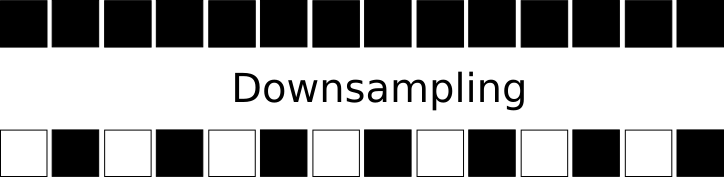
\includegraphics[width=0.4\linewidth]{images/downsampling}
						\label{fig:downsampling}
						\\Fonte: Elaborado pelo autor, 2023.
					\end{figure}
				
			\subsection{Caracterização dos processos de produção da voz humana}
				\par A fala possui três grandes áreas de estudo: A fisiológica, também conhecida como fonética articulatória, a acústica, referida como fonética acústica, e ainda, a perceptual, que cuida da percepção  da  fala \cite{kremer2014eficiencia}. Neste trabalho, o foco será apenas na questão acústica, pois não serão analisados aspectos da fisiologia relacionada à voz, mas sim os sinais sonoros propriamente ditos.
				
				\subsubsection{Sinais vozeados \textit{versus} não-vozeados}
				
					\par Quando da análise dos sinais de voz, consideram-se as partes vozeadas e não-vozeadas. Aquelas são produzidas com a ajuda da vibração quase periódica das pregas vocais, enquanto estas praticamente não contam com participação regrada da referida estrutura.
				
				\subsubsection{Frequência fundamental da voz}
					\par Também conhecida como $F_0$, é o componente periódico resultante da vibração das pregas vocais. Em termos de percepção, se pode interpretar $F_0$ como o tom da voz, isto é, a frequência de \textit{pitch} \cite{kremer2014eficiencia}. Vozes agudas tem uma frequência de \textit{pitch} alto, enquanto vozes mais graves tem baixa. A alteração da frequência (jitter) e/ou intensidade (shimmer) do \textit{pitch} durante a fala é definida como entonação,  porém, também pode indicar algum distúrbio ou doença relacionada ao trato vocal \cite{WERTZNER2005}.
					
					\par A frequência fundamental da voz é o número de vezes na qual uma forma de onda característica, que reflete a excitação pulmonar moldada pelas pregas vocais, se repete por unidade de tempo. Sendo assim, as medidas de $F_0$ geralmente são apresentadas em Hz \cite{freitas2013avaliaccao}.
					
					\par A medição de $F_0$ está sujeita a contaminações surgidas das variações naturais de \textit{pitch} típicas da voz humana \cite{freitas2013avaliaccao}. A importância de se medir $F_0$ corretamente vem do fato de que, além de carregar boa parte da informação da fala, ela é a base para construção das outras frequências que compõe os sinais de voz, que são múltiplas de $F_0$.
				
				\subsubsection{Formantes}
					\par O sinal de excitação que atravessa as pregas vocais é rico em harmônicas, isto é, frequências múltiplas da fundamental. Tais harmônicas podem ser atenuadas ou amplificadas, em função da estrutura dos tratos vocal e nasal de cada locutor. Particularmente, o primeiro formante ($F_1$), relaciona-se à  amplificação  sonora  na  cavidade  oral  posterior  e  à  posição  da  língua  no  plano  vertical;  o segundo  formante  ($F_2$)  à  cavidade  oral  anterior  e  à  posição  da  língua  no  plano  horizontal; o terceiro  formante  ($F_3$)  relaciona-se  às  cavidades  à  frente  e  atrás  do  ápice  da  língua e, finalmente,  o  quarto formante  ($F_4$) relaciona-se  ao  formato  da  laringe  e  da  faringe  na  mesma  altura  \cite{valencca2014analise}. Formantes caracterizam fortemente os locutores, pois cada indivíduo possui um formato de trato vocal e nasal. Assim, tais frequências, que podem ser capturadas com ferramentas diversas, a exemplo da Transformada \textit{Wavelet}, são de suma importância na área de verificação de locutores.
				
				\subsection{Escalas e energias dos sinais}
					\par A energia de um sinal digital $s[\cdot]$ com $M$ amostras é definida como
					
					\begin{equation}
						E = \sum\limits_{i=0}^{M-1}(s_i)^2 \qquad.   
					\end{equation}
				
					$E$ pode ainda sofrer normalizações e ter a sua mensuração restrita a uma parte específica do sinal sob análise. Possibilidades para tais restrições podem, por exemplo, envolver a escala BARK \cite{doi:10.1121-1.1908630} e MEL \cite{beranek1949acoustic} que serão utilizadas neste trabalho.
					\subsubsection{A escala BARK}
						\par BARK foi definida tendo em mente vários tipos de sinais acústicos. Essa escala corresponde ao conjunto de 25 bandas críticas da audição humana. Suas frequências-base de audiometria são, em Hz: \textbf{20, 100, 200, 300, 400, 510, 630, 770, 920, 1080, 1270, 1480, 1720, 2000, 2320, 2700, 3150, 3700, 4400, 5300, 6400, 7700, 9500, 12000, 15500}. Nessa escala,os sinais digitais no domínio temporal atravessam filtros passa-faixas \cite{bosi2002introduction} para os quais o início e o final da banda de passagem correspondem à frequências-base consecutivas resultando em um vetor de características com 24 coeficientes e, em seguida, as energias dos sinais filtrados são utilizadas como características descritivas de propriedades do sinal sob análise, como mostrado na Figura \ref{fig:barkfeaturevect}.
						\begin{figure}[h]
							\centering
							\caption{Cálculo de vetores de características com BARK}
							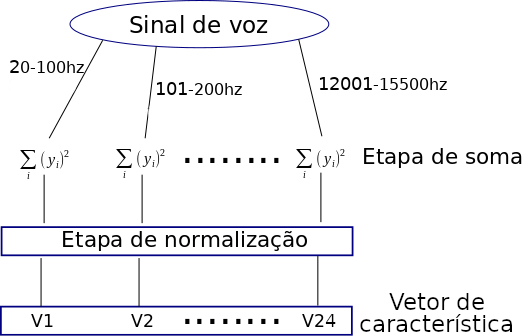
\includegraphics[width=0.6\linewidth]{images/barkFeatureVect}
							\label{fig:barkfeaturevect}
							\\Fonte: Elaborado pelo autor, 2023.
						\end{figure}
					\subsubsection{A escala MEL}
						\par Escala Mel, advinda do termo \textit{melody}, é uma adaptação da escala Bark para sinais de voz. Dentre as várias implementações de bandas críticas a escolhida foi a implementação que contém os valores em Hz: \textbf{20, 160, 394, 670, 1000, 1420, 1900, 2450, 3120, 4000, 5100, 6600, 9000, 14000}.
						
						\par A variante que será usada neste trabalho é conhecida como \textit{Mel-frequency cepstral coefficients}(MFCC) a qual inclui, além dos intervalos definidos, uma diminuição da correlação entre os componentes gerados via aplicação da Transformada Discreta Cosseno (DCT) \cite{salomon2007data} ou da Análise de Componentes Principais (PCA) \cite{jolliffe2006principal} seguida de duas derivações no vetor de características resultando em um total de 11 coeficientes. Nesse trabalho foi escolhida a DCT, no entanto, PCA poderia também ser escolhida sem prejuízos, o uso de uma ou outra depende da preferência do autor.
						
						\par Novamente, desconsiderando qualquer etapa intermediária que possa ser adicionada, as energias calculadas nos intervalos definidos na escala MEL podem, por si mesmas, constituir um vetor de características, como mostrado na Figura \ref{fig:barkfeaturevect}.
						
						\begin{figure}[h]
							\centering
							\caption{Cálculo de vetores de características com MEL}
							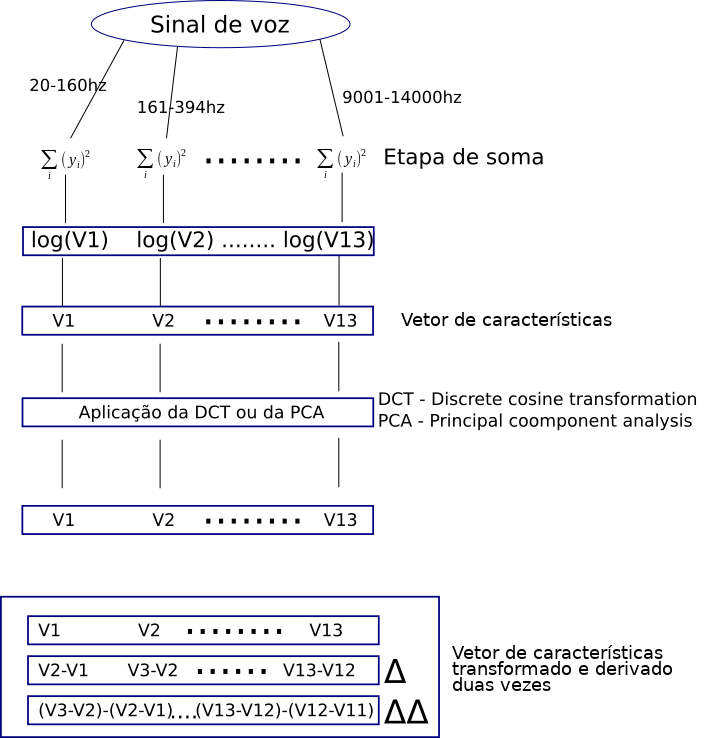
\includegraphics[width=0.8\linewidth]{images/melFeatureVect}
							\label{fig:melfeaturevect}
							\\Fonte: Elaborado pelo autor, 2023.
						\end{figure}
				
					\subsection{Filtros digitais \textit{wavelet}}
						\par Filtros digitais \textit{wavelet} têm sido utilizados com sucesso para suprir as deficiências de janelamento de sinal apresentadas pelas Transformadas de Fourier e de Fourier de Tempo Reduzido. \textit{Wavelets} contam com variadas funções-filtro e têm tamanho de janela variável, o que permite uma análise multirresolução \cite{Rod5254905}. Particularmente, as \textit{wavelets} proporcionam a análise do sinal de forma detalhada tanto no espectro de baixa frequência quanto no de alta contando com diferentes funções-base não periódicas diferentemente da tradicional transformada de Fourrier que utilizam somente as bases periódicas senoidal e cossenoidal.
						
						\par É importante observar que, quando se trata de Transformadas \textit{Wavelet}, seis elementos estão presentes: dois filtros de análise, dois filtros de síntese e as funções ortogonais \textit{scaling} e \textit{wavelet}. No tocante a sua aplicação, só a transformada direta, e não a inversa, será usada na construção dos vetores de características. Portanto, os filtros de síntese, a função \textit{scaling} e a função \textit{wavelet} não serão elementos abordados aqui: eles somente interessariam caso houvesse a necessidade da transformada inversa.
						
						\par No contexto dos filtros digitais baseados em \textit{wavelets}, o tamanho da janela recebe o nome de \textbf{suporte}. Janelas definem o tamanho do filtro que será aplicado ao sinal. Quando esse é pequeno (limitado), se diz que a janela tem \textbf{um suporte compacto} \cite{robi2003}.
						
						\par Se diz que uma \textit{wavelet} tem boa \textbf{resposta em frequência} quando, na aplicação da mesma para filtragem, não são causadas muitas pertubações indesejadas ao sinal, no domínio da frequência. Os filtros \textit{wavelet} de Daubechies \cite{daubechies1992ten} se destacam nesse quesito por serem \textit{maximamente planos} (\textit{maximally-flat}) \cite{butterworth1930} \cite{bianchi2007electronic} nos platôs de resposta em frequência como indicado na Figura \ref{fig:daubechies} ao contrário do que ocorre na Figura \ref{fig:nomaximallyflat}.
						
						\begin{figure}[h]
							\centering
							\caption{Platôs maximamente planos em um filtro digital: característica da família de Daubechies}
							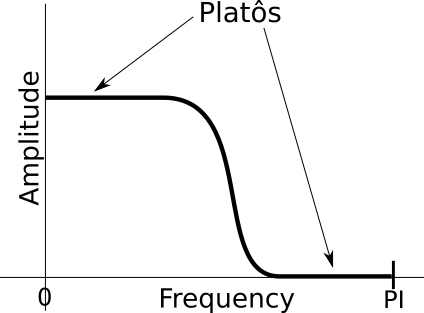
\includegraphics[width=0.3\linewidth]{images/daubechies}
							\label{fig:daubechies}
							\\Fonte: Elaborado pelo autor, 2023.
						\end{figure}
						
						\begin{figure}[h]
							\centering
							\caption{Platôs não maximamente planos de um filtro digital: características de outros filtros \textit{wavelet}, distintos da família de Daubechies}
							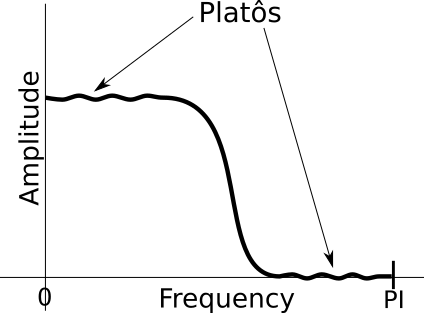
\includegraphics[width=0.3\linewidth]{images/noMaximallyFlat}
							\label{fig:nomaximallyflat}
							\\Fonte: Elaborado pelo autor, 2023.
						\end{figure}
						
						\par Além da resposta em frequência, na aplicação de um filtro digital \textit{wavelet} também é possível considerar a \textbf{resposta em fase}, que constitui um atraso ou adiantamento do sinal filtrado em relação ao sinal original, ambos no domínio temporal. Esse deslocamento pode ser \textbf{linear}, \textbf{quase linear} ou \textbf{não linear}: 
						
						\begin{itemize}
							\item na resposta em fase \textbf{linear}, há o mesmo deslocamento de fase para todos os componentes do sinal;
							\item quando a resposta em fase é \textbf{quase linear} existe uma pequena diferença no deslocamento dos diferentes componentes do sinal;
							\item finalmente, quando a resposta é \textbf{não linear}, acontece um deslocamento significativamente heterogêneo para as diferentes frequências que compõe o sinal.
						\end{itemize}
						
						\par Idealmente, é desejável que todo filtro apresente boa resposta em frequência e em fase linear. Características de fase e frequência de algumas famílias de filtros \textit{wavelet} constam na Tabela \ref{tab:waveletsProperties}.
						
						\begin{table}[h]
	\centering
	\caption{Algumas das \textit{wavelets} mais usadas e suas propriedades}
	\begin{tabular}{|c|p{75mm}|c|}
			\hline 
			\textbf{Wavelet} & \textbf{Resposta em frequência} & \textbf{Resposta em fase} \\ 
			\hline 
			Haar & Pobre &  Linear \\ 
			\hline 
			Daubechies & mais próxima da ideal à medida que o \newline  suporte aumenta; \textit{maximally-flat}  &  Não linear \\ 
			\hline 
			Symmlets & mais próxima da ideal à medida que o \newline  suporte aumenta; não \textit{maximally-flat}  & Quase linear \\ 
			\hline 
			Coiflets & mais próxima da ideal à medida que o \newline  suporte aumenta; não \textit{maximally-flat}  & Quase linear \\ 
			\hline 
	\end{tabular} 
	\label{tab:waveletsProperties}
	\\Fonte: Elaborado pelo autor, 2023.
\end{table}

				
						\subsubsection{O algoritmo de Mallat para a Transformada \textit{Wavelet}}
							\par Baseando-se no artigo \citetext{7079589}, percebe-se que algoritmo de Mallat faz com que aplicação das \textit{wavelets} seja uma simples multiplicação de matrizes. O sinal que deve ser transformado se torna uma matriz linear vertical. Os filtros passa-baixa e passa-alta tornam-se, nessa ordem, linhas de uma matriz quadrada que será completada segundo regras que serão mostradas mais adiante. É importante que essa matriz quadrada tenha a mesma dimensão que o sinal a ser transformado.
							
							\par Interessantemente, para que seja possível a transformação \textit{wavelet}, basta ter disponível o vetor do filtro passa-baixas calculado a partir da \textit{mother wavelet}, que é a função geradora desse filtro, já que o passa-alta pode ser construído a partindo-se da ortogonalidade do primeiro.
							
							\par Determinar a ortogonal de um vetor significa construir um vetor, tal que, o produto escalar do vetor original com sua respectiva ortogonal seja nulo.
							
							\par Considerando $h[\cdot]$ como sendo o vetor do filtro passa-baixas e $g[\cdot]$ seu correspondente ortogonal, tem-se que $h[\cdot] \cdot g[\cdot] = 0 \qquad .$
							\par Portanto, se $h[\cdot]=[a, b, c, d]$ então seu ortogonal será $g[\cdot]=[d, -c, b, -a]$ pois:
							$$
							h[\cdot] \cdot g[\cdot]  =  [a, b, c, d] \cdot [d, -c, b, -a] = (a \cdot d) + (b \cdot (-c)) + (c \cdot b) + (d \cdot (-a)) = ad - ad + bc - bc = 0 \qquad.
							$$
							
							\par A título de exemplo, considera-se:
							\begin{itemize}
								\item o filtro passa baixa baseado na \textit{wavelet} Haar: $h[\cdot] = [\frac{1}{\sqrt{2}}, \frac{1}{\sqrt{2}}]$
								\item o seu respectivo vetor ortogonal: $g[\cdot] = [\frac{1}{\sqrt{2}}, \frac{-1}{\sqrt{2}}]$
								\item e também o seguinte sinal-exemplo de entrada: $s = \{1,2,3,4\}$
							\end{itemize}
							
							\par Se o tamanho do sinal a ser tratado é quatro e se pretende-se aplicar o filtro Haar, a seguinte matriz de coeficientes é construída:
							\begin{equation}
								\begin{pmatrix}
									\frac{1}{\sqrt{2}}, \frac{1}{\sqrt{2}}, 0, 0\\
									\frac{1}{\sqrt{2}}, \frac{-1}{\sqrt{2}}, 0, 0\\
									0, 0, \frac{1}{\sqrt{2}}, \frac{1}{\sqrt{2}}\\
									0, 0, \frac{1}{\sqrt{2}}, \frac{1}{\sqrt{2}}
									\label{eq:haarFilters}
								\end{pmatrix} 
							\end{equation}
							\par Tendo em vista que a dimensão do sinal sob análise é diferente da dimensão do filtro, basta completar cada uma das linhas da matriz de coeficientes com zeros. A matriz é montada de forma que ela seja ortogonal.
							
							\par Montada a matriz de filtros, segue-se com os cálculos da transformada:
							\begin{equation}
								\begin{pmatrix}
									\frac{1}{\sqrt{2}}, \frac{1}{\sqrt{2}}, 0, 0\\
									\frac{1}{\sqrt{2}}, \frac{-1}{\sqrt{2}}, 0, 0\\
									0, 0, \frac{1}{\sqrt{2}}, \frac{1}{\sqrt{2}}\\
									0, 0, \frac{1}{\sqrt{2}}, \frac{1}{\sqrt{2}}\\
								\end{pmatrix} 
								\cdot
								\begin{pmatrix}
									1\\
									2\\
									3\\
									4\\
								\end{pmatrix} 
								=
								\begin{pmatrix}
									\frac{3}{\sqrt{2}}\\
									\frac{-1}{\sqrt{2}}\\
									\frac{7}{\sqrt{2}}\\
									\frac{-1}{\sqrt{2}}
								\end{pmatrix}
								\label{eq:haarMultiplic}
							\end{equation}
							
							\par Realizada a multiplicação, é necessário montar o sinal filtrado. Isso é feito escolhendo, dentro do resultado, valores alternadamente de forma que o vetor resultante seja:
							
							\begin{equation}
								resultado = \Big[
								\frac{3}{\sqrt{2}},
								\frac{7}{\sqrt{2}},
								\frac{-1}{\sqrt{2}},
								\frac{-1}{\sqrt{2}}
								\Big]\qquad.
								\label{eq:haarResult}
							\end{equation}
							
							\par Percebe-se que, na transformação descrita nas Equações \ref{eq:haarFilters}, \ref{eq:haarMultiplic} e \ref{eq:haarResult}, a \textbf{aplicação dos filtros sobre o vetor de entrada ocorreu apenas uma vez}. Sendo assim, se diz que o sinal recebeu uma \textbf{transformação de nível 1}. A cada transformação, há uma separação do sinal em dois componentes: o de baixa e o de alta frequência.
							
							\par Embora haja um limite, que será mencionado adiante, é possível aplicar mais de um nível de decomposição ao sinal. Para que se possa fazer isso, a Transformada \textit{Wavelet} nível 2 deve considerar apenas a parte de baixas frequências da primeira transformada; a transformada de nível 3 deve considerar apenas a parte de baixas frequências da transformada nível 2, e assim consecutivamente.
							
							\par Nos exemplos numéricos mostrados nas Tabelas \ref{tab:regularWaveletExample}, \ref{tab:packetWaveletExampleLF} e \ref{tab:packetWaveletExampleHF}, usou-se um filtro normalizado cujos coeficientes são $\{\dfrac{1}{2},-\dfrac{1}{2}\}$. Os dados destacados em \textbf{verde} correspondem ao \textbf{vetor original} que será tratado. Cada uma das linhas são os resultados das transformações nos níveis 1, 2, 3 e 4, respectivamente. As partes em \textbf{azul} correspondem à porção de \textbf{baixas frequências}, enquanto que as partes em \textbf{amarelo} correspondem às porções de \textbf{altas frequências}.
							
							\par Percebe-se que na Tabela \ref{tab:regularWaveletExample}, a partir da transformação nível 2, apenas as partes de baixa frequência são modificadas. Isso implica que, no momento da implementação do algoritmo de Mallat \textbf{para níveis maiores que 1}, a abordagem será \textbf{recursiva}. Em outras palavras, a partir do nível 1 se deve aplicar Mallat apenas às porções de baixas-frequências geradas pela transformação anterior.
							
							\begin{table}[h]
	\fontsize{9}{\baselineskip} \selectfont
	\newcommand{\mc}[3]{\multicolumn{#1}{#2}{#3}}
	\definecolor{tcA}{rgb}{0.65098,0.65098,0.65098}
	\definecolor{tcD}{rgb}{1,0.94902,0}
	\definecolor{tcC}{rgb}{0,0.5,1}
	\definecolor{tcB}{rgb}{0.447059,0.74902,0.266667}
	\begin{center}
		\caption{Exemplo numérico da transformação \textit{wavelet} aplicada a um vetor}
		\begin{tabular}{c|ccccccccccccccc|c}
			% use packages: color,colortbl
			\mc{1}{>{\columncolor{tcA}}c|}{\textbf{Sinal}} & \mc{1}{>{\columncolor{tcB}}c}{\textbf{32}} & \mc{1}{>{\columncolor{tcB}}c}{\textbf{10}} & \mc{1}{>{\columncolor{tcB}}c}{\textbf{20}} & \mc{1}{>{\columncolor{tcB}}c}{\textbf{38}} & \mc{1}{>{\columncolor{tcB}}c}{\textbf{37}} & \mc{1}{>{\columncolor{tcB}}c}{\textbf{28}} & \mc{1}{>{\columncolor{tcB}}c}{\textbf{38}} & \mc{1}{>{\columncolor{tcB}}c}{\textbf{34}} & \mc{1}{>{\columncolor{tcB}}c}{\textbf{18}} & \mc{1}{>{\columncolor{tcB}}c}{\textbf{24}} & \mc{1}{>{\columncolor{tcB}}c}{\textbf{24}} & \mc{1}{>{\columncolor{tcB}}c}{\textbf{9}} & \mc{1}{>{\columncolor{tcB}}c}{\textbf{23}} & \mc{1}{>{\columncolor{tcB}}c}{\textbf{24}} & \mc{1}{>{\columncolor{tcB}}c}{\textbf{28}} & \mc{1}{>{\columncolor{tcB}}c}{\textbf{34}}\\
			\hline
			
			\mc{1}{>{\columncolor{tcA}}c|}{Nível 01} & \mc{1}{>{\columncolor{tcC}}c}{21} & \mc{1}{>{\columncolor{tcC}}c}{29} & \mc{1}{>{\columncolor{tcC}}c}{32,5} & \mc{1}{>{\columncolor{tcC}}c}{36} & \mc{1}{>{\columncolor{tcC}}c}{21} & \mc{1}{>{\columncolor{tcC}}c}{16,5} & \mc{1}{>{\columncolor{tcC}}c}{23,5} & \mc{1}{>{\columncolor{tcC}}c}{31} & \mc{1}{>{\columncolor{tcD}}c}{11} & \mc{1}{>{\columncolor{tcD}}c}{-9} & \mc{1}{>{\columncolor{tcD}}c}{4,5} & \mc{1}{>{\columncolor{tcD}}c}{2} & \mc{1}{>{\columncolor{tcD}}c}{-3} & \mc{1}{>{\columncolor{tcD}}c}{7,5} & \mc{1}{>{\columncolor{tcD}}c}{-0,5} & \mc{1}{>{\columncolor{tcD}}c}{-3}\\
			\hline
			
			\mc{1}{>{\columncolor{tcA}}c|}{Nível 02} & \mc{1}{>{\columncolor{tcC}}c}{25} & \mc{1}{>{\columncolor{tcC}}c}{34,25} & \mc{1}{>{\columncolor{tcC}}c}{18,75} & \mc{1}{>{\columncolor{tcC}}c}{27,25} & \mc{1}{>{\columncolor{tcD}}c}{-4} & \mc{1}{>{\columncolor{tcD}}c}{-1,75} & \mc{1}{>{\columncolor{tcD}}c}{2,25} & \mc{1}{>{\columncolor{tcD}}c}{-3,75} & \mc{1}{>{\columncolor{tcD}}c}{11} & \mc{1}{>{\columncolor{tcD}}c}{-9} & \mc{1}{>{\columncolor{tcD}}c}{4,5} & \mc{1}{>{\columncolor{tcD}}c}{2} & \mc{1}{>{\columncolor{tcD}}c}{-3} & \mc{1}{>{\columncolor{tcD}}c}{7,5} & \mc{1}{>{\columncolor{tcD}}c}{-0,5} & \mc{1}{>{\columncolor{tcD}}c}{-3}\\
			\hline
			
			\mc{1}{>{\columncolor{tcA}}c|}{Nível 03} & \mc{1}{>{\columncolor{tcC}}c}{29,62} & \mc{1}{>{\columncolor{tcC}}c}{23} & \mc{1}{>{\columncolor{tcD}}c}{-4,625} & \mc{1}{>{\columncolor{tcD}}c}{-4,25} & \mc{1}{>{\columncolor{tcD}}c}{-4} & \mc{1}{>{\columncolor{tcD}}c}{-1,75} & \mc{1}{>{\columncolor{tcD}}c}{2,25} & \mc{1}{>{\columncolor{tcD}}c}{-3,75} & \mc{1}{>{\columncolor{tcD}}c}{11} & \mc{1}{>{\columncolor{tcD}}c}{-9} & \mc{1}{>{\columncolor{tcD}}c}{4,5} & \mc{1}{>{\columncolor{tcD}}c}{2} & \mc{1}{>{\columncolor{tcD}}c}{-3} & \mc{1}{>{\columncolor{tcD}}c}{7,5} & \mc{1}{>{\columncolor{tcD}}c}{-0,5} & \mc{1}{>{\columncolor{tcD}}c}{-3}\\
			\hline
			
			\mc{1}{>{\columncolor{tcA}}c|}{Nível 04} & \mc{1}{>{\columncolor{tcC}}c}{26,3125} & \mc{1}{>{\columncolor{tcD}}c}{3,3125} & \mc{1}{>{\columncolor{tcD}}c}{-4,625} & \mc{1}{>{\columncolor{tcD}}c}{-4,25} & \mc{1}{>{\columncolor{tcD}}c}{-4} & \mc{1}{>{\columncolor{tcD}}c}{-1,75} & \mc{1}{>{\columncolor{tcD}}c}{2,25} & \mc{1}{>{\columncolor{tcD}}c}{-3,75} & \mc{1}{>{\columncolor{tcD}}c}{11} & \mc{1}{>{\columncolor{tcD}}c}{-9} & \mc{1}{>{\columncolor{tcD}}c}{4,5} & \mc{1}{>{\columncolor{tcD}}c}{2} & \mc{1}{>{\columncolor{tcD}}c}{-3} & \mc{1}{>{\columncolor{tcD}}c}{7,5} & \mc{1}{>{\columncolor{tcD}}c}{-0,5} & \mc{1}{>{\columncolor{tcD}}c}{-3}
		\end{tabular}
		\label{tab:regularWaveletExample}
		\fontsize{12}{\baselineskip} \selectfont
		\\Fonte: Elaborado pelo autor, 2023.
	\end{center}
\end{table}
				
						\subsubsection{O algoritmo de Mallat e a Transformada \textit{Wavelet-Packet}}
							\par Na Transformada \textit{Wavelet-Packet}, os filtros aplicados são os mesmos da Transformada \textit{Wavelet} e o procedimento recursivo de cálculo também é o mesmo, no entanto, realizada a transformação de nível 1, a transformada de nível 2 deve ser aplicada aos componentes de baixa e de alta frequência. Sendo assim a Transformada \textit{Wavelet-Packet} obtém um nível de detalhes em todo o espectro de frequência, maior do que uma transformação regular. 
							
							\par Os exemplos mostrados nas Tabelas \ref{tab:packetWaveletExampleLF} e \ref{tab:packetWaveletExampleHF} permitem perceber como se dão as transformações na porção de \textbf{baixa} e de \textbf{alta} frequências, respectivamente, após a transformação \textit{wavelet-packet} de nível 1, 2, 3 e 4.
							
							\par Devido ao \textit{downsampling} aplicado às porções de alta frequência, essas partes acabam por ficar ``espelhadas'' no espectro \cite{Jensen_2001}, ou seja, suas sequências ficam invertidas. Para resolver esse problema e preservar a ordem das sub-bandas no sinal transformado, os filtros são aplicados em ordem inversa nas porções de alta frequência. Isso altera como o algoritmo de Mallat deve ser implementado para a Transformada \textit{Wavelet-Packet}, já que dessa vez é preciso se atentar a ordem da aplicação dos filtros passa-alta e passa-baixa.
							
							\begin{table}[h]
	\newcommand{\mc}[3]{\multicolumn{#1}{#2}{#3}}
	\definecolor{tcA}{rgb}{0.65098,0.65098,0.65098}
	\definecolor{tcD}{rgb}{1,0.94902,0}
	\definecolor{tcC}{rgb}{0,0.5,1}
	\definecolor{tcB}{rgb}{0.447059,0.74902,0.266667}
	\begin{center}
		\caption{Exemplo numérico de \textit{wavelet-packet} Haar aplicada ao vetor da Tabela \ref{tab:regularWaveletExample} (porção das baixas frequências)}
		\begin{tabular}{l|llllllll|}
			% use packages: color,colortbl
			\mc{1}{>{\columncolor{tcA}}l|}{\textbf{Sinal}} & \mc{1}{>{\columncolor{tcB}}l}{\textbf{32}} & \mc{1}{>{\columncolor{tcB}}l}{\textbf{10}} & \mc{1}{>{\columncolor{tcB}}l}{\textbf{20}} & \mc{1}{>{\columncolor{tcB}}l}{\textbf{38}} & \mc{1}{>{\columncolor{tcB}}l}{\textbf{37}} & \mc{1}{>{\columncolor{tcB}}l}{\textbf{28}} & \mc{1}{>{\columncolor{tcB}}l}{\textbf{38}} & \mc{1}{>{\columncolor{tcB}}l|}{\textbf{34}}\\
			\hline
			
			\mc{1}{>{\columncolor{tcA}}l|}{Nivel 01} & \mc{1}{>{\columncolor{tcC}}l}{21} & \mc{1}{>{\columncolor{tcC}}l}{29} & \mc{1}{>{\columncolor{tcC}}l}{32,5} & \mc{1}{>{\columncolor{tcC}}l}{36} & \mc{1}{>{\columncolor{tcC}}l}{21} & \mc{1}{>{\columncolor{tcC}}l}{16,5} & \mc{1}{>{\columncolor{tcC}}l}{23,5} & \mc{1}{>{\columncolor{tcC}}l|}{31}\\
			\hline
			
			\mc{1}{>{\columncolor{tcA}}l|}{Nivel 02} & \mc{1}{>{\columncolor{tcC}}l}{25} & \mc{1}{>{\columncolor{tcC}}l}{34,25} & \mc{1}{>{\columncolor{tcC}}l}{18,75} & \mc{1}{>{\columncolor{tcC}}l|}{27,25} & \mc{1}{>{\columncolor{tcD}}l}{-4} & \mc{1}{>{\columncolor{tcD}}l}{-1,75} & \mc{1}{>{\columncolor{tcD}}l}{2,25} & \mc{1}{>{\columncolor{tcD}}l|}{-3,75}\\
			\hline
			
			\mc{1}{>{\columncolor{tcA}}l|}{Nivel 03} & \mc{1}{>{\columncolor{tcC}}l}{29,62} & \mc{1}{>{\columncolor{tcC}}l|}{23} & \mc{1}{>{\columncolor{tcD}}l}{-4,625} & \mc{1}{>{\columncolor{tcD}}l|}{-4,25} & \mc{1}{>{\columncolor{tcD}}l}{-1,125} & \mc{1}{>{\columncolor{tcD}}l|}{3} & \mc{1}{>{\columncolor{tcC}}l}{-2,875} & \mc{1}{>{\columncolor{tcC}}l|}{-0,75}\\
			\hline
			
			\mc{1}{>{\columncolor{tcA}}l|}{Nivel 04} & \mc{1}{>{\columncolor{tcC}}l|}{26,3125} & \mc{1}{>{\columncolor{tcD}}l|}{3,3125} & \mc{1}{>{\columncolor{tcD}}l|}{-0,1875} & \mc{1}{>{\columncolor{tcC}}l|}{-4,4375} & \mc{1}{>{\columncolor{tcC}}l|}{0,9375} & \mc{1}{>{\columncolor{tcD}}l|}{-2,0625} & \mc{1}{>{\columncolor{tcD}}l|}{-1,0625} & \mc{1}{>{\columncolor{tcC}}l|}{-1,8125}\\
		\end{tabular}
		\label{tab:packetWaveletExampleLF}
		\\Fonte: Elaborado pelo autor, 2023.
	\end{center}
\end{table}

\begin{table}[h]
	\newcommand{\mc}[3]{\multicolumn{#1}{#2}{#3}}
	\definecolor{tcA}{rgb}{0.65098,0.65098,0.65098}
	\definecolor{tcC}{rgb}{1,0.94902,0}
	\definecolor{tcD}{rgb}{0,0.5,1}
	\definecolor{tcB}{rgb}{0.447059,0.74902,0.266667}
	\begin{center}
		\caption{Exemplo numérico de \textit{wavelet-packet} Haar aplicada ao vetor da Tabela \ref{tab:regularWaveletExample} (porção das altas frequências)}
		\begin{tabular}{c|cccccccc}
			% use packages: color,colortbl
			\mc{1}{>{\columncolor{tcA}}c|}{\textbf{Sinal}} & \mc{1}{>{\columncolor{tcB}}c}{\textbf{18}} & \mc{1}{>{\columncolor{tcB}}c}{\textbf{24}} & \mc{1}{>{\columncolor{tcB}}c}{\textbf{24}} & \mc{1}{>{\columncolor{tcB}}c}{\textbf{9}} & \mc{1}{>{\columncolor{tcB}}c}{\textbf{23}} & \mc{1}{>{\columncolor{tcB}}c}{\textbf{24}} & \mc{1}{>{\columncolor{tcB}}c}{\textbf{28}} & \mc{1}{>{\columncolor{tcB}}c|}{\textbf{34}}\\\hline
			\mc{1}{>{\columncolor{tcA}}c|}{Nivel 01} & \mc{1}{>{\columncolor{tcC}}c}{11} & \mc{1}{>{\columncolor{tcC}}c}{-9} & \mc{1}{>{\columncolor{tcC}}c}{4,5} & \mc{1}{>{\columncolor{tcC}}c}{2} & \mc{1}{>{\columncolor{tcC}}c}{-3} & \mc{1}{>{\columncolor{tcC}}c}{7,5} & \mc{1}{>{\columncolor{tcC}}c}{-0,5} & \mc{1}{>{\columncolor{tcC}}c|}{-3}\\\hline
			\mc{1}{>{\columncolor{tcA}}c|}{Nivel 02} & \mc{1}{>{\columncolor{tcC}}c}{10} & \mc{1}{>{\columncolor{tcC}}c|}{1,25} & \mc{1}{>{\columncolor{tcC}}c}{-5,25} & \mc{1}{>{\columncolor{tcC}}c|}{1,25} & \mc{1}{>{\columncolor{tcD}}c}{1} & \mc{1}{>{\columncolor{tcD}}c|}{3,25} & \mc{1}{>{\columncolor{tcD}}c}{2,25} & \mc{1}{>{\columncolor{tcD}}c|}{-1,75}\\\hline
			\mc{1}{>{\columncolor{tcA}}c|}{Nivel 03} & \mc{1}{>{\columncolor{tcD}}c|}{5,625} & \mc{1}{>{\columncolor{tcD}}c|}{-2} & \mc{1}{>{\columncolor{tcC}}c|}{4,375} & \mc{1}{>{\columncolor{tcC}}c|}{-3,25} & \mc{1}{>{\columncolor{tcC}}c|}{-1,125} & \mc{1}{>{\columncolor{tcC}}c|}{2} & \mc{1}{>{\columncolor{tcD}}c|}{2,125} & \mc{1}{>{\columncolor{tcD}}c|}{0,25}\\\hline
			
			\mc{1}{>{\columncolor{tcA}}c|}{Nivel 04} & \mc{1}{>{\columncolor{tcD}}c|}{1,8125} & \mc{1}{>{\columncolor{tcC}}c|}{3,8125} & \mc{1}{>{\columncolor{tcC}}c|}{3,8125} & \mc{1}{>{\columncolor{tcD}}c|}{0,5625} & \mc{1}{>{\columncolor{tcD}}c|}{0,4375} & \mc{1}{>{\columncolor{tcC}}c|}{-1,5625} & \mc{1}{>{\columncolor{tcC}}c|}{0,9375} & \mc{1}{>{\columncolor{tcD}}c|}{1,1875}\\
		\end{tabular}
		\label{tab:packetWaveletExampleHF}
		\\Fonte: Elaborado pelo autor, 2023.
	\end{center}
\end{table}
				
				\subsection{Engenharia Paraconsistente de características}
					\par Nos processos de classificação, frequentemente surge a questão: ``Os vetores de características criados proporcionam uma boa separação de classes?''. A Engenharia Paraconsistente de Características, recém publicada \cite{8588433}, que usa a paraconsistência \cite{da1998elementos},  \cite{COSTA2000} é, em meio a outras técnicas, uma ferramenta que pode ser usada para responder essa questão.
					
					\par O processo inicia-se após a aquisição dos vetores de características para cada classe $C_n$. Se o número de classes presentes for, por exemplo, quatro então estas poderão ser representadas por $C_1, C_2, C_3, C_4$.
					\par Em seguida é necessário o cálculo de duas grandezas:
					
					\begin{itemize}
						\item a menor similaridade intraclasse, $\alpha$.
						\item a razão de sobreposição interclasse, $\beta$.
					\end{itemize}
					
					\par $\alpha$ indica o quanto de similaridade os dados têm entre si, dentro de uma mesma classe, enquanto $\beta$ é a razão de sobreposição entre diferentes classes. Idealmente, $\alpha$ deve ser maximizada e $\beta$ minimizada para que classificadores extremamente modestos apresentem uma acurácia interessante.
					
					\par Particularmente, para calcular $\alpha$ e $\beta$, é necessária a normalização dos vetores de características de forma que todos os seus componentes estejam no intervalo entre $0$ e $1$. Em seguida, a obtenção de $\alpha$ se dá selecionando-se os maiores e os menores valores de cada uma das posições de todos os vetores de características para cada classe, gerando assim um vetor para os valores maiores e outro para os menores.
					
					\par O \textbf{vetor de similaridade da classe}$(svC_n)$ é obtido fazendo-se a diferença item-a-item dos maiores em relação aos menores. Finalmente, e para cada classe, é obtida a média dos valores para cada vetor de similaridade, sendo que $\alpha$ é o menor valor dentre essas médias. A Figura \ref{fig:calculoalpha} contém uma ilustração do processo.
					
					\begin{figure}[h]
						\centering
						\caption{Cálculo do coeficiente $\alpha$.}
						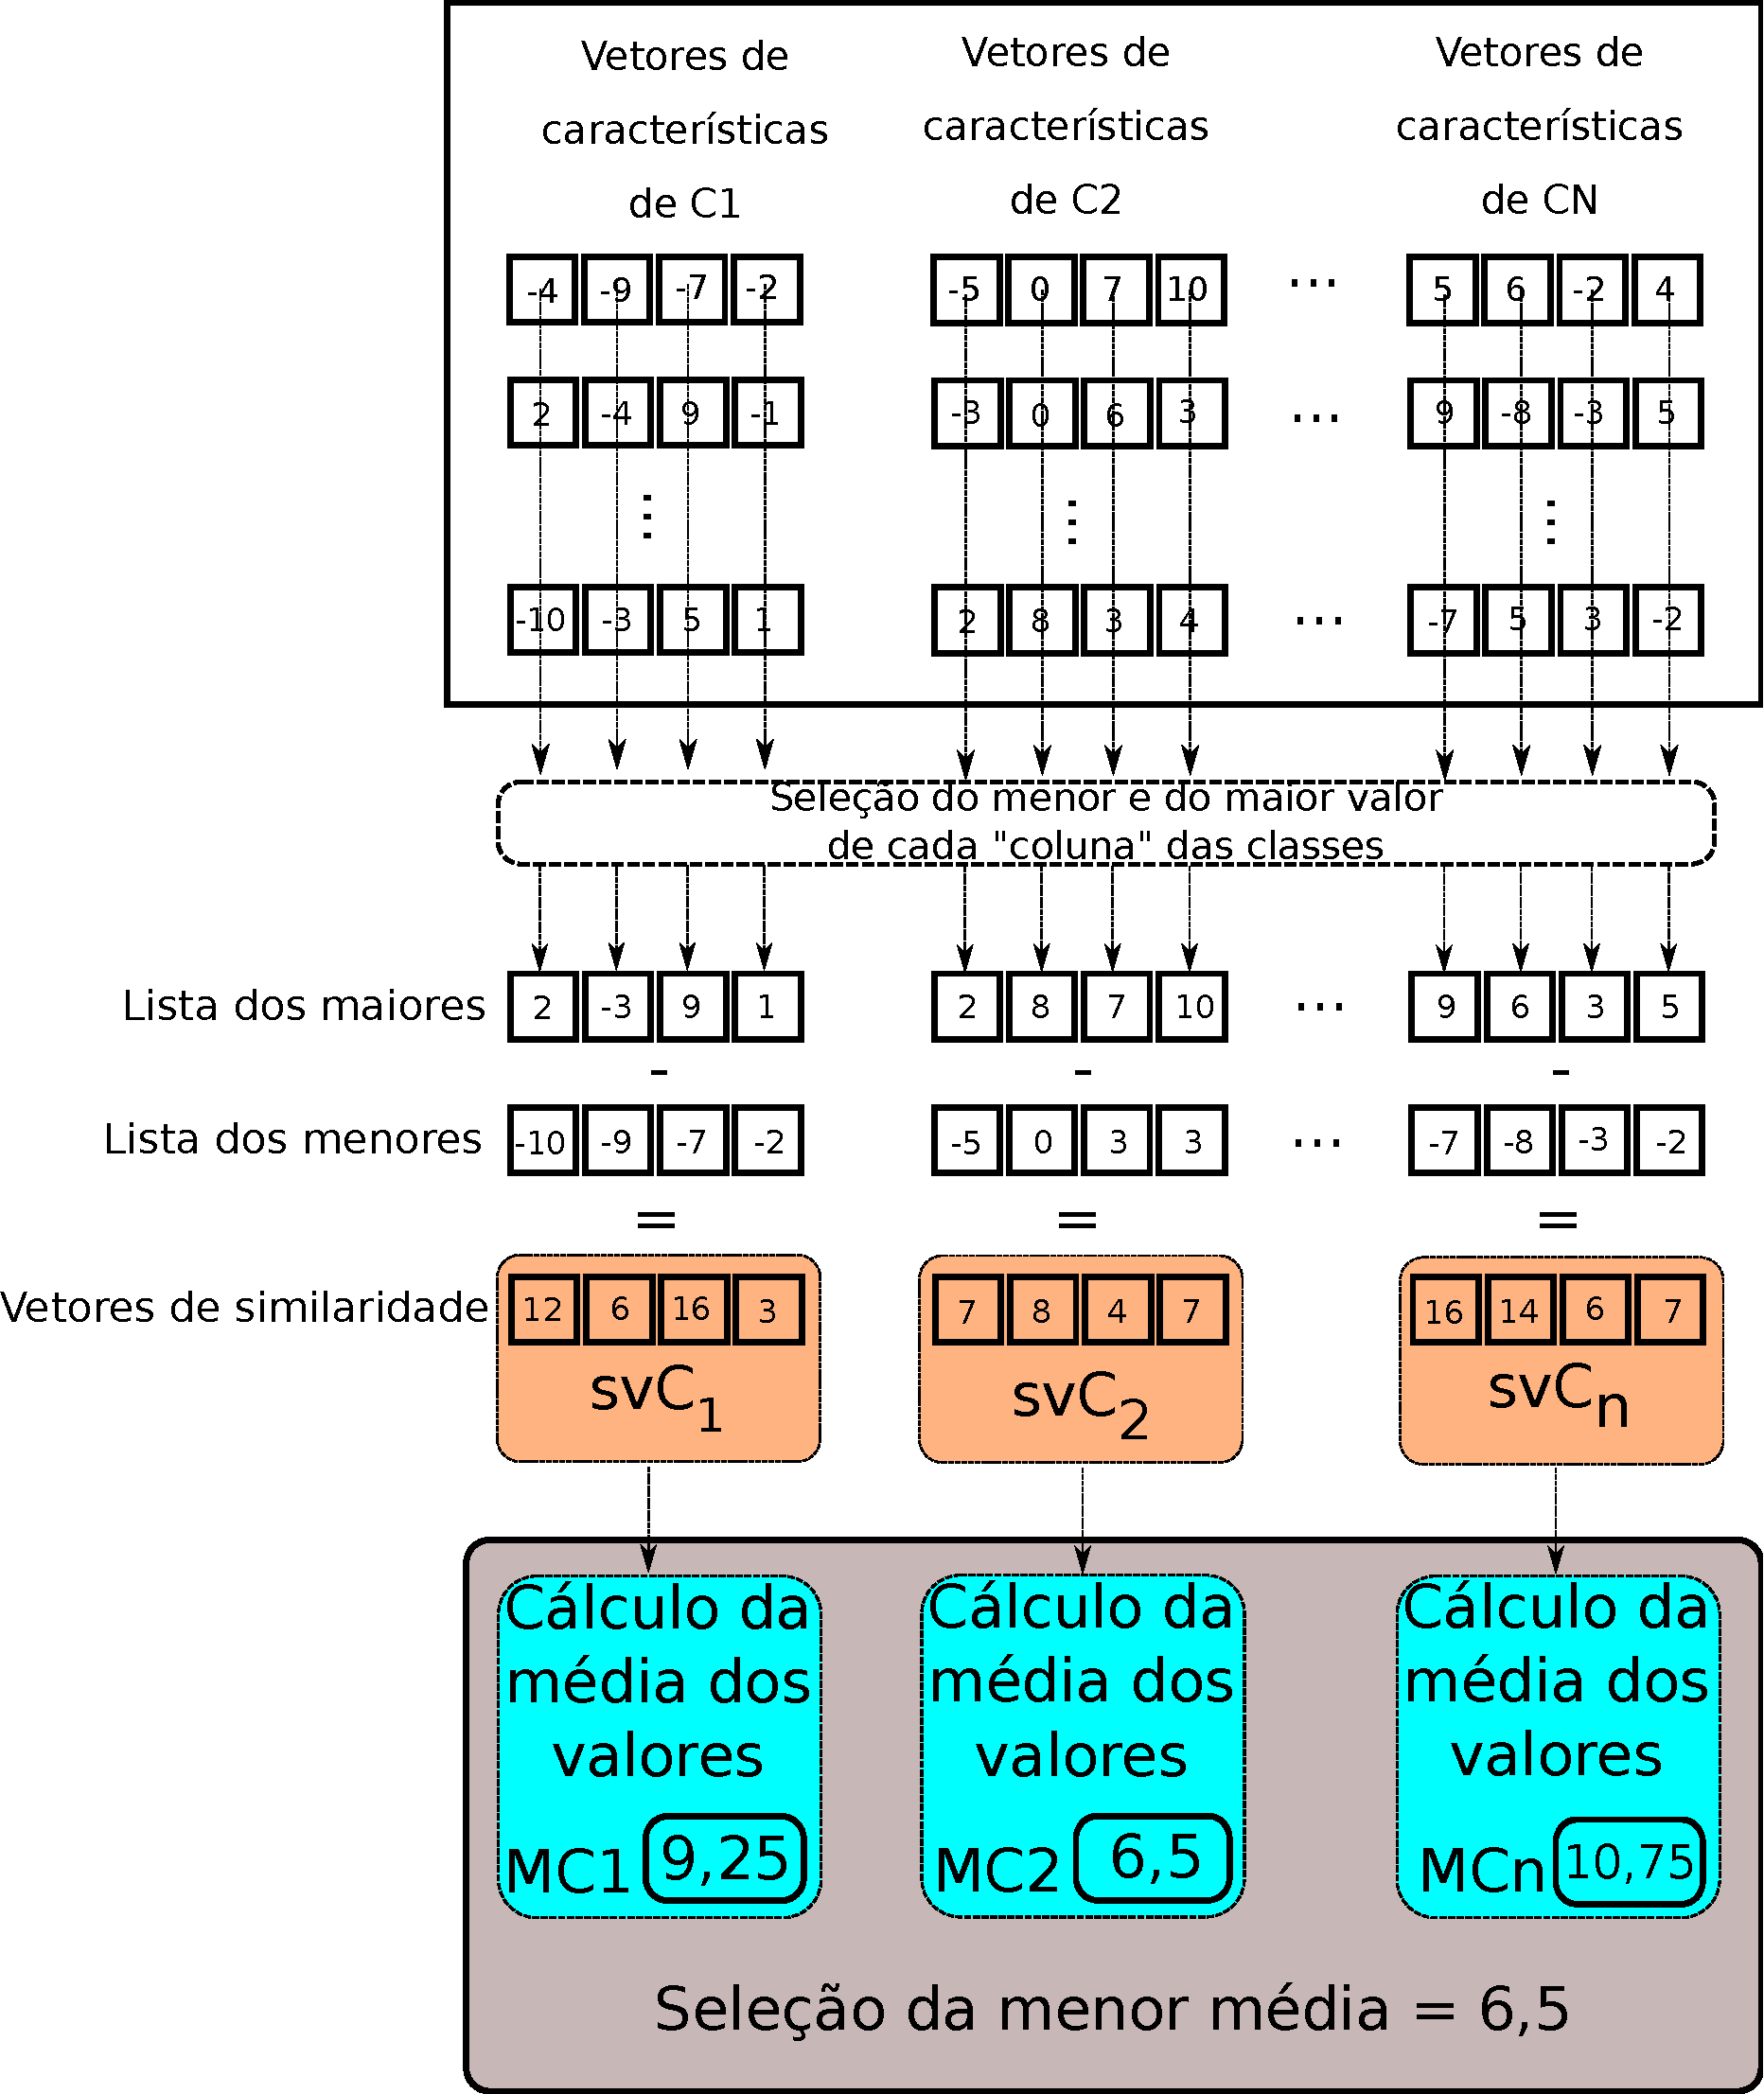
\includegraphics[width=0.5\linewidth]{images/calculoAlpha.pdf}
						\label{fig:calculoalpha}
						\\Fonte: Adaptado de \cite{8588433}.
					\end{figure}
					
					\par A obtenção de $\beta$, assim como ilustrado na Figura \ref{fig:betacalculation}, também se dá selecionando os maiores e os menores valores de cada uma das posições de todos os vetores de características de cada classe, gerando assim um vetor para os valores maiores e outro para os menores.
					
					\par Na sequência, realiza-se o cálculo de $R$ cujo valor é a quantidade de vezes que um valor do vetor de características de uma classe se encontra entre os valores maiores e menores de outra classe.
					
					\par Seja:
					\begin{itemize}
						\item N a quantidades de classes;
						\item X a quantidade de vetores de características por classe;
						\item T o tamanho do vetor de características.
					\end{itemize}
					
					\par Então, $F$, que é o número máximo de sobreposições possíveis entre classes, é dado por:
					\begin{equation}
						F=N.(N-1).X.T \qquad.
					\end{equation}
					\par Finalmente, $\beta$ é calculado da seguinte forma:
					\begin{equation}
						\beta=\dfrac{R}{F} \qquad.
					\end{equation}
					
					\par Neste ponto, é importante notar que $\alpha=1$ sugere fortemente que os vetores de características de cada classe são similares e representam suas respectivas classes precisamente. Complementarmente, $\beta=0$ sugere os vetores de características de classes diferentes não se sobrepõe \cite{8588433}.
					
					\begin{figure}[h]
						\centering
						\caption{Cálculo de $\beta$: Os itens destacados em azul e rosa são aqueles pertencentes a classe C1 e CN que se sobrepõe, em verde, a sobreposição é entre C1 e C2. Para cada sobreposição verificada soma-se 1 ao valor $R$. Essa comparação é feita para todos os vetores de características de cada uma das classes.}
						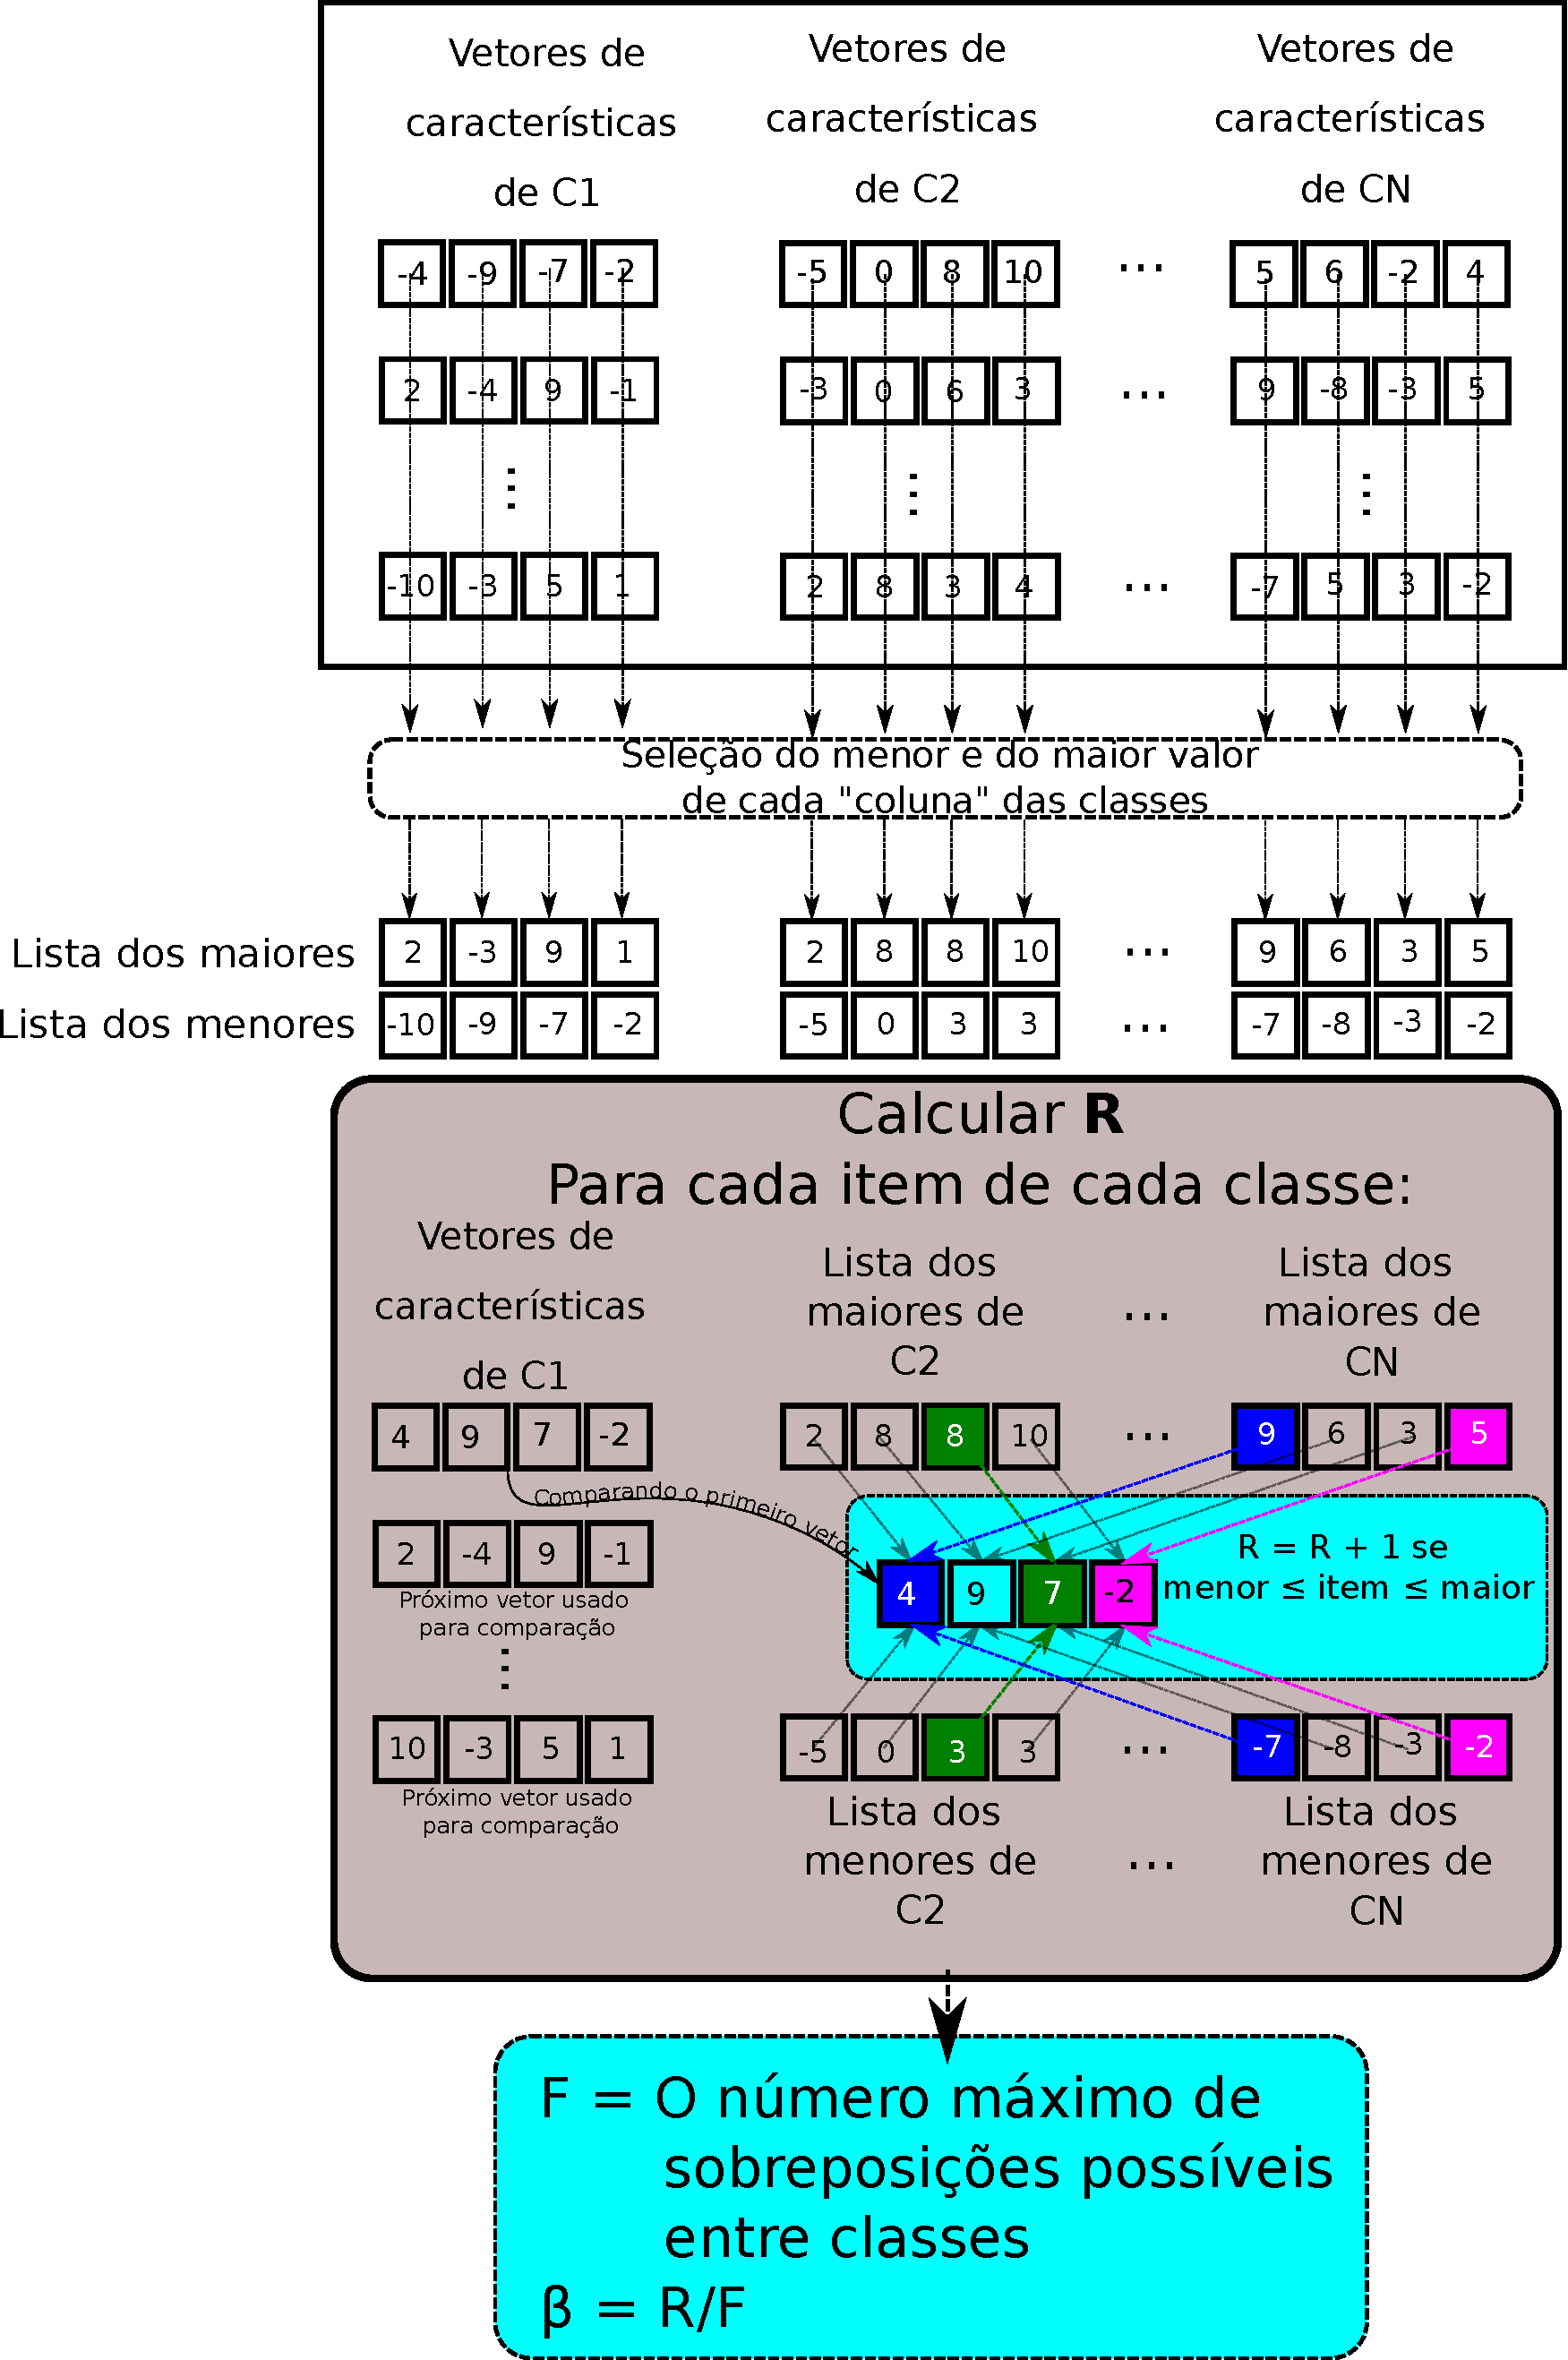
\includegraphics[width=0.5\linewidth]{images/betaCalculation.pdf}
						\label{fig:betacalculation}
						\\Fonte: Adaptado de \cite{8588433}.
					\end{figure}
					
					\par Considerando-se o plano paraconsistente \cite{8588433}, temos: 
					
					\begin{itemize}
						\item Verdade $\rightarrow$ fé total ($\alpha = 1$) e nenhum descrédito ($\beta = 0$)
						\item Ambiguidade $\rightarrow$ fé total ($\alpha = 1$) e descrédito total ($\beta = 1$)
						\item Falsidade $\rightarrow$ fé nula ($\alpha = 0$) e descrédito total ($\beta = 1$)
						\item Indefinição $\rightarrow$ fé nula ($\alpha = 0$) e nenhum descrédito ($\beta = 0$) \qquad.
					\end{itemize}
					
					\par No entanto, raramente $\alpha$ e $\beta$ terão valores inteiros como os mostrados na listagem acima: Na maioria das ocasiões, $0 \leqslant \alpha \leqslant 1$ e $0 \leqslant \beta \leqslant 1$. Por isso, se torna necessário o cálculo do \textbf{grau de certeza}, isto é, $G_1$, e do \textbf{grau de contradição}, isto é, $G_2$, conforme segue:
					\begin{equation}
						G_1=\alpha-\beta  \qquad,
					\end{equation}
					\begin{equation}
						G_2=\alpha+\beta-1 \qquad,
					\end{equation}
					onde: $-1 \leqslant G_1$ e  $1 \geqslant G_2$.
					
					\par Os valores de $G_1$ e $G_2$, em conjunto, definem os graus entre verdade ($G_1=1$) e falsidade ($G_1=-1$) e também os graus entre indefinição ($G_2=-1$) e ambiguidade ($G_2=1$). Novamente, raramente tais valores inteiros serão alcançados já que $G_1$ e $G_2$ dependem de $\alpha$ e $\beta$.
					
					\par O Plano Paraconsistente, para fins de visualização e maior rapidez na avaliação dos resultados, encontra-se ilustrado na Figura \ref{fig:paraconsistentplane} e tem quatro arestas precisamente definidas:
					\begin{itemize}
						\item (-1,0) $\rightarrow$ falsidade;
						\item (1,0) $\rightarrow$ verdade;
						\item (0,-1) $\rightarrow$ indefinição;
						\item (0,1) $\rightarrow$ ambiguidade.
					\end{itemize}
					\par A propósito de ilustração na Figura \ref{fig:paraconsistentplane}, é possível ver um pequeno círculo indicando os graus dos quatro casos listados.
					
					\par Para se ter ideia em que área exatamente se encontram as classes avaliadas, as distâncias $(D)$ do ponto $P=(G_1,G_2)$ até o limites supracitados podem ser computadas. Tais cálculos podem ser feitos da seguinte forma:
					
					\begin{equation}
						D_{-1,0}=\sqrt{(G_1+1)^2+(G_2)^2}\qquad,
					\end{equation}
					\begin{equation}
						D_{1,0}=\sqrt{(G_1-1)^2+(G_2)^2}\qquad,
					\end{equation}
					\begin{equation}
						D_{0,-1}=\sqrt{(G_1)^2+(G_2+1)^2}\qquad,		
					\end{equation}
					\begin{equation}
						D_{0,1}=\sqrt{(G_1)^2+(G_2-1)^2}\qquad.
					\end{equation}		
					
					\begin{figure}[H]
						\centering
						\caption{O plano paraconsistente: O pequeno círculo indica os graus de falsidade(-1,0), verdade(1,0), indefinição(0,-1) e ambiguidade(0,1)}
						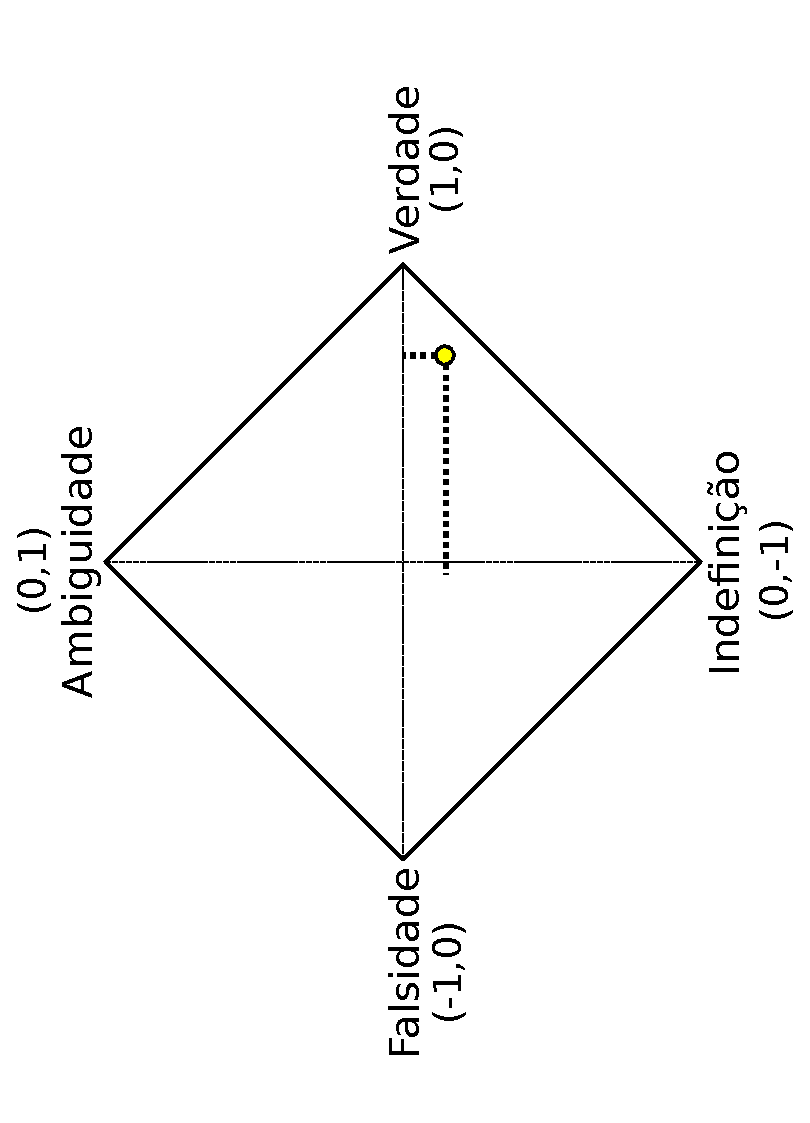
\includegraphics[angle=-90, width=0.69\linewidth]{images/paraconsistentPlane.pdf}
						\label{fig:paraconsistentplane}
						\\Fonte: Adaptado de \cite{8588433}.
					\end{figure}
					\par Na prática, ou seja, para fins de classificação, geralmente considera-se a distância em relação ao ponto \textit{``(1,0) $\rightarrow$ Verdade''}, que é o ponto ótimo: quanto mais próximo o ponto $(G_1,G_2)$ estiver de $(1,0)$, mais as os vetores de características das diferentes classes estão naturalmente separados. Isso implica, dentro da limitação de cada algoritmo, em resultados melhores sejam quais forem os classificadores usados.
					
				\subsection{Redes neurais}
					\subsubsection{Autoencoders}
					
					\par Como ilustrado na Figura \ref{fig:autoencoder} \textit{Autoencoders} são redes neurais treinadas para reconstruir seus dados de entrada. Eles consistem em uma função codificadora, denotada como $h = f(x)$, e uma função decodificadora que produz uma reconstrução, denotada como $r = g(h)$. A camada oculta $h$ representa um código ou representação comprimida da entrada \cite{Goodfellow-et-al-2016}. \newline
					
					\par O principal objetivo de um \textit{autoencoder} é aprender uma representação compactada dos dados de entrada na camada oculta e, em seguida, reconstruir os dados de entrada com a maior precisão possível usando o decodificador. No entanto, os \textit{autoencoders} são projetados para serem incapazes de copiar perfeitamente os dados de entrada. Eles geralmente são limitados de alguma forma para apenas aproximar a entrada e priorizar certos aspectos dos dados. \newline
					
					\par \textit{Autoencoders} podem ser treinados usando várias técnicas, como \textit{gradient descent} com \textit{minibatch} ou estocástico \cite{Goodfellow-et-al-2016}.
					
					\begin{figure}[h]
						\centering
						\caption[autoencoder]{\textit{Autoencoder}: $x$ é codificado para uma dimensão menor $h$ e, em seguida, é reconstruído em $r$, tal processo pode implicar ou não em uma perda na reconstrução}
						\begin{tikzpicture}[node distance=1.5cm, every edge/.style={draw=black,->}]
							% Nodes
							\node[draw, circle] (x) {$x$};
							\node[draw, rectangle, above right=0.7cm and 1cm of x] (encoder) {Codificador};
							\node[draw, circle, above right=0.7cm and 1cm of encoder] (h) {$h$};
							\node[draw, rectangle, below right=0.7cm and 1cm of h] (decoder) {Decodificador};
							\node[draw, circle, below right=0.7cm and 1cm of decoder] (r) {$r$};
							
							% Arrows
							\draw (x) edge (encoder);
							\draw (encoder) edge (h);
							\draw (h) edge (decoder);
							\draw (decoder) edge (r);
							
							% Loss
							\node[below of=h, yshift=-0.7cm] (loss) {Perda na reconstrução};
							\draw (x) edge (loss);
							\draw (r) edge (loss);
							
							% Labels
							\node[below of=x, yshift=0.7cm] {Entrada};
							\node[below right=0.2cm and 0.8cm of decoder] {Decoder};
							\node[below of=r, yshift=0.7cm] {Entrada reconstruida};
						\end{tikzpicture}
						\label{fig:autoencoder}
					\end{figure}
				
					\par Considerando-se que a reconstrução $r$ seja razoável, isso significa que a região $h$  contém dados suficientes para representar a informação em sua essência, sendo assim, dentro do contexto das redes neurais, autoencoders são ótimos produtores de vetores de características.
					
					\subsubsection{Redes neurais residuais (ResNets)}
						\par Segundo \cite{DBLP:journals/corr/HeZRS15} a ideia-chave por trás do \textit{ResNets} é a inclusão de conexões de salto como ilustrado na Figura \ref{fig:residualblock}, também conhecidas como mapeamentos de identidade, que permitem que a saída de uma camada seja adicionada diretamente à entrada da camada subsequente. Isso contorna as camadas intermediárias e garante que redes mais profundas possam aprender. Outra vantagem no uso de conexões de salto é que essa prática diminui a ocorrência de \textit{vanishing gradients} um problema comum em redes com muitas camadas que pode impossibilitar ou diminuir a níveis impraticáveis o aprendizado da rede.
						
						\begin{figure}
							\centering
							\caption[bloco de uma Resnet]{Bloco de uma Rede Neural Residual, $X$ é uma função identidade que contorna as camada intermediárias criando "\textit{highway connections}"}
							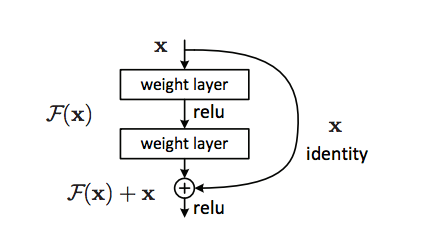
\includegraphics[width=0.7\linewidth]{images/residualBlock}
							\\ Fonte: \cite{DBLP:journals/corr/HeZRS15}
							\label{fig:residualblock}
						\end{figure}
						
					\subsubsection{\textit{Spike Neural Networks}}
						\par Em \cite{kasabov2018time} se define uma \textit{Spike Neural Network},com um tipo de rede neural artificial inspirada na maneira como os neurônios se comunicam no cérebro por meio do uso de picos ou potenciais de ação. Nesse tipo de rede as informações são representadas pelo tempo e pela taxa de picos, e não pela força das conexões entre os neurônios.
						
						\par Seu modo de operação pode ser altamente paralelo com, potencialmente, todos os neurônios operando em paralelo
					
						\par Nas SNNs, o tempo dos picos e a dinâmica temporal da rede desempenham um papel crucial no processamento da informação pois cada pico carrega informações de tempo, permitindo uma codificação mais precisa de informações e comunicação assíncrona entre os neurônios.
					
						\par Em se tratando do estudo atual e considerando a natureza temporal do sinais de voz e EEG, hipotéticamente, as SNNs são promissoras para classificação de tais informações.					
				
			\section{Trabalhos correlatos}
				\label{sec:trabcorrelatos}
		
				\par O estudo \cite{WOS:000841879504172} avaliou um grupo de 432 falantes da língua inglesa de variadas etnias e deficiências na fala coletando amostras e metainformações. Uma rede extratora de características composta por 8 camadas e uma rede \textit{Long Short-Term Memory}(LSTM) classificadora de 2 foram treinadas com as falas. A entrada para o sistema ASR são as energias calculadas a partir de um banco de filtros para 80 dimensões. Os resultados superaram os transcritores humanos com ganhos médios e máximos de precisão de reconhecimento de 9\% e 80\%, respectivamente. A precisão dos modelos foi alta, com uma taxa de erro de palavras (WER) média de 4,6\%\newline
				
				\par  Em \cite{jin21_interspeech} se discute os desafios de reconhecer a fala disfônica e a importância das técnicas de aumento de dados no desenvolvimento de sistemas automáticos de reconhecimento de fala (ASR). Devido à complexidade das condições neuromotoras e deficiências físicas que acompanham a fala disfônica, é difícil coletar uma grande quantidade de amostras para treinar os sistemas ASR. O estudo propõe uma abordagem de aumento de dados usando redes adversariais generativas de convolução profunda (DCGAN) para modelar diferenças espectro-temporais detalhadas entre a fala disfônica e a fala normal. Experimentos realizados na base UASpeech demonstram que essa abordagem de aumento de dados supera consistentemente os métodos de aumento existentes baseados em perturbação de tempo ou velocidade, alcançando uma redução da taxa de erro de palavra (WER) de até 3,05\% em comparação com o sistema de referência sem aumento de dados.\newline
				
				\par O estudo \cite{WOS:000614122200021} teve como objetivo desenvolver um sistema para detectar segmentos de palavras imaginadas em sinais EEG contínuos usando diferentes conjuntos de características e classificadores. Os pesquisadores testaram cinco conjuntos de características baseados em Transformada Discreta de Wavelet (DWT), Decomposição Empírica de Modos (EMD), características de energia, dimensões fractais e medidas de caos. Esses conjuntos de características foram usados para treinar quatro classificadores: Random Forest (RF), Support Vector Machine (SVM), K-Nearest Neighbors (KNN) e Logistic Regression (LR). A avaliação de desempenho utilizou-se do \textit{F1 score} \cite{tharwat2020classification} e obteve um pontuação média de 0,75. Mais informações sobre o \textit{F1 score} na Seço \ref{sec:f1scoresec}.\newline
				
				\par Aqui se apresenta um sistema de Reconhecimento Automático de Fala (ASR) que combina sinais de áudio e sinais de Eletroencefalograma (EEG) para aprimorar o reconhecimento de fala em sistemas de Interação Humano-Máquina (HMI) \cite{WOS:000591530700001}. O estudo explora o uso de múltiplas modalidades e aplica técnicas de Transformada Wavelet (WT) para extrair informações de fala dos sinais.	Os resultados alcançam taxas de precisão de até 74,48\%.\newline
	
				\par Nesta revisão \cite{WOS:000857544900001} se examinou o uso de técnicas de inteligência artificial (IA) para decodificar a fala a partir de sinais cerebrais humanos, especificamente usando dados de eletroencefalografia (EEG). Os resultados da revisão indicaram o seguinte:
				
				\begin{itemize}
					\item Modalidade de Dados e Técnicas de IA: Os estudos analisaram o uso de dados de eletroencefalografia (EEG) e estímulos de palavras/frases. As técnicas de inteligência artificial (IA) utilizadas foram principalmente aprendizado de máquina e aprendizado profundo. Máquinas de vetores de suporte (SVM) e análise discriminante linear (LDA) foram comumente empregadas no aprendizado de máquina, enquanto redes neurais convolucionais (CNN) e redes neurais artificiais foram amplamente utilizadas no aprendizado profundo.
					
					\item Extração de Características e Processamento de Sinais: Devido ao ruído presente nos sinais de EEG, foram aplicadas técnicas de normalização e extração de características adequadas. A filtragem de banda passante, combinada com outras técnicas de normalização, foi frequentemente utilizada. As técnicas de extração de características incluíram padrões espaciais comuns, características estatísticas simples (como mínimo, máximo e média) e transformações discretas de wavelet.
					
					\item Conjunto de Dados e Equipamentos de Gravação: A maioria dos estudos utilizou dispositivos de EEG com 64 canais para capturar os sinais cerebrais, embora um estudo tenha utilizado um dispositivo de 128 canais. Alguns estudos empregaram dispositivos com 32 canais ou menos.
				\end{itemize}
	
				\par O artigo \cite{salim2023automatic} propõe um sistema de verificação automática de falas (ASV) para pacientes com disartria usando recursos prosódicos (pitch, volume e probabilidade de vocalização) e aumento de dados fora do domínio. O estudo utilizou dois bancos de dados, a saber, o \textit{Dyarthric Speech Database} (DSD) e o banco de dados \textit{SpeechDat-Car}. Foram gerados vetores de características i-vector e x-vector usando MFCC (Mel-frequency cepstral coefficients), variáveis prosódicas e suas combinações. A combinação de MFCC, recursos de prosódia e aumento de dados produziu um EER de 11,09 para disartria leve, 13,26 na media e 11,97 para disartria grave.\newline
	
				\par O artigo \cite{6296526} discute o uso de redes neurais profundas (DNNs) como criadores de modelos acústicos. Modelagem acústica é o processo de vinculação entre unidades linguísticas (como fonemas, palavras ou sentenças) e sinais de áudio. Neste artigo as DNNs são usadas para geração de vetores de características para posterior classificação usando \textit{Hidden Markov Models} (HMM). Em relação a base dedos usada, a escolhida foi \textit{TIMIT} que consiste em gravações de mais 630 falantes da língua inglesa. Essa combinação (DNN + HMM) atingiu uma WER de 18,5\%.\newline
				
				\par Em \cite{abderrazek20_interspeech} a base de dados \textit{BREF} é composta por registros de fala francesa produzidos por 120 falantes, a mesma foi elaborada para fornecer falas contínuas para o desenvolvimento e avaliação de sistemas de Reconhecimento Automático de Fala e para modelagem de variação fonológica. Além dessa base uma própria (C2SI-LEC) contendo pacientes com falas disfuncionais também foi incluída. O artigo usou um modelo de Rede Neural Convolucional (CNN) para classificação. As características extraídas do sinal de fala foram os Coeficientes Cepstrais de Frequência Mel (MFCCs) e suas primeiras e segundas derivadas. Os dados de entrada foram normalizados subtraindo-se a média e dividindo-se pelo desvio padrão. Para lidar com a distribuição desproporcional das classes, uma técnica de subamostragem aleatória foi adotada durante a fase de treinamento. Uma taxa de aprendizado inicial de 0,001 seguindo um cronograma de decaimento exponencial e uma estratégia de parada antecipada foi utilizada para o treinamento da CNN. O classificador acurácia de 0,68 na base \textit{BREF} e 0,71 na base \textit{C2SI-LEC}, os ouvintes humanos foram superados em ambas as bases.\newline
				
				\par No artigo \cite{pawar2022wavelet}, para obtenção dos dados foram usados 8 canais de EEG para medição dos sinais nos participantes. Múltiplas características foram extraídas simultaneamente desses sinais de EEG usando a transformadas Wavelets em cada um dos canais. Uma rede neural recorrente de memória de curto prazo (LSTM-RNN) foi usada para decodificar os sinais de EEG correspondentes a quatro comandos de áudio: para cima, para baixo, para a esquerda e para a direita. O artigo relata que o reconhecimento de padrões alcançou uma acurácia de classificação geral de 92,50\%. Outras métricas como precisão, \textit{recall} e \textit{F1-score} também foram consideradas obtendo-se 92,74\%, 92,50\% e 92,62\% respectivamente.\newline
				
				\par Em \cite{cooney2021bimodal} utilizou-se dados de EEG e espectroscopia de infravermelho próximo funcional (fNIRS) para coleta dos dados. Tais informações foram então separadas na categoria de tempo (média, variância, assimetria e curtose) e frequência (densidade espectral de potência e potência de banda). Os recursos extraídos foram então usados para treinar classificadores como o de análise discriminante linear (LDA), máquina de vetores de suporte (SVM) e uma rede neural convolucional (CNN). Alcançou-se uma precisão de classificação de 87,18\% para fala aberta e de 53\% para fala imaginada principalmente quando os estímulos foram imagens.\newline
				
				\par Neste estudo \cite{bakhshali2022investigating} registrou-se sinais de EEG correspondentes a fala imaginada de quatro vogais vindas de oito voluntários. Esse dados foram codificados em matrizes que representam a conectividade funcional entre diferentes regiões do cérebro durante a fala imaginada, de onde extraiu-se onze características afim de se detectar interações entre regiões com base no índice de localização. O índice de localização é definido como LI = NS/NT, onde NS é o número de conexões significativas entre as regiões e NT é o número total de conexões entre as regiões. Os classificadores usados foram uma SVM e a Análise Discriminante Linear (LDA). A precisão média da classificação foi de 81,1\%.\newline
				
				\par O artigo \cite{lee2021decoding} propõe uma estrutura baseada em aprendizado métrico profundo para decodificar a \textit{imagined speech} usando interfaces cérebro-máquina (BCI). O método proposto foi avaliado em duas bases dados: o banco de dados \textit{Coretto} contendo 6 classes e a base \textit{BCI Competition} com 5 classes. Os sinais de EEG foram medidos durante a fala imaginada, e a frequência instantânea e entropia espectral foram extraídas dos sinais. A estrutura proposta usa uma rede neural siamesa que aprende a perda contrastante com base na distância determinada por uma estrutura de aprendizagem métrica profunda. O classificador obteve um precisão dentre 6 classes de 45,00 ± 3,13\% e uma entre de 5 classes de 48,10 ± 3,68\%.\newline
	
				\par Aqui \cite{tamm2020classification} se usou um conjunto de dados EEG com 15 sujeitos imaginando dizer cinco vogais (a, e, i, o, u) e seis palavras diferentes. Após a coleta, visando melhorar a etapa de classificação, os dados passaram por uma etapa de pré-processamento que incluiu os seguintes procedimentos:
				\begin{itemize}
					\item filtragem passa-faixa entre $0,5Hz$ e $100Hz$ para remover quaisquer frequências indesejadas.
					\item subamostragem para 100 Hz afim de reduzir a carga computacional.
					\item segmentação em lotes de 2 segundos, com uma sobreposição de 1 segundo entre os sinais.
					\item normalização para média zero e variância unitária.
				\end{itemize}
				Em se tratando de classificadores foi usada uma rede neural convolucional com transferência de aprendizado para classificar os sinais correspondentes às falas imaginadas atingindo uma acurácia de 23.98\% (±3.08).\newline
				
				\par Segundo \cite{8396208} \textit{Hashing} sensível a locus(LSH) é frequentemente usado como um classificador para problemas relacionados a \textit{big data}, neste trabalho é proposto uma junção de MFCC e LSH a fim de se reconhecer o locutor. Neste método o MFCC é extraído dos arquivos de sinal para posterior aplicação do LSH gerando assim uma tabela \textit{hash}, estes valores de \textit{hash} são então comparados identificando assim o locutor ou locutora. Nos testes realizados houve uma acurácia de 92,66\%. A base de dados usada foi a \textit{TIMIT 2018} \cite{TIMIT2018}.
				
				
				\subsection{Fechamento}
				
					\par Com base nos estudos mencionados nesta pesquisa, pretende-se utilizar uma camada extratora de características semelhante à abordada por \cite{WOS:000841879504172}, bem como a aplicação de filtros wavelet packet para a decomposição dos sinais. Além disso, considera-se a possibilidade de recorrer a técnicas de aumento de dados, como aquelas empregadas por \cite{jin21_interspeech}, devido à escassez de locutores disfônicos.
					
					\par No estudo de \cite{tamm2020classification}, é apresentado um protocolo para a obtenção de dados (Figura \ref{fig:recordingprotocol}), o qual pode ser utilizado diretamente ou adaptado para esta pesquisa. Nesse mesmo estudo, menciona-se uma base de dados chamada UASpeech, que pode fornecer informações valiosas para a verificação de padrões.
					
					\par Dentre os artigos revisados, \cite{WOS:000614122200021} parece ter a menor relevância em relação às ideias abordadas, uma vez que o método de extração de dados já está definido, ao contrário, o trabalho de \cite{WOS:000591530700001} se aproxima mais da proposta desta pesquisa, uma vez que utiliza diretamente as Transformadas Wavelet para a criação dos vetores de características.
					
					\par No estudo de \cite{WOS:000857544900001}, são discutidas técnicas interessantes de normalização de dados que talvez possam ser utilizadas.
					
					Embora os coeficientes MFCC (Mel-frequency cepstral coefficients), mencionados em \cite{furlan2021caracterizacao} e \cite{salim2023automatic}, não tenham apresentado melhorias nos vetores de características, a utilização de técnicas de aumento de dados fora do domínio, mencionada em \cite{salim2023automatic}, pode ser útil.
					
					\par Embora o artigo citado \cite{6296526} não se aplique diretamente ao problema desta tese, ele apresenta o conceito de Modelagem Acústica.
					
					\par Já em \cite{bakhshali2022investigating} o conceito de matrizes que representam a conectividade funcional entre diferentes regiões do cérebro durante a fala imaginada parece promissor e talvez possa ajudar a produzir novas intuições acerca dos padrão cerebrais dado que, segundo o próprio estudo, diferentes regiões do cérebro são ativadas durante as falas imaginadas.
					
					\par Outro estudo relevante é o de \cite{lee2021decoding}, que propõe uma estrutura baseada em aprendizado métrico profundo para decodificar a fala imaginada. No entanto, essa abordagem difere significativamente da proposta desta pesquisa.
					
					\par Em resumo, nenhum dos artigos analisados utiliza as técnicas propostas neste estudo, tais como autoencoders, redes neurais residuais, spike neural networks e vetores de características "hand-crafted". Além disso, nenhum deles tem como objetivo comparar esses métodos, o que torna esta tese potencialmente relevante para a comunidade acadêmica.
				
				\begin{figure}
					\centering
					\caption[Protocolo de obtenção]{Protocolo para a obtenção de dados.}
					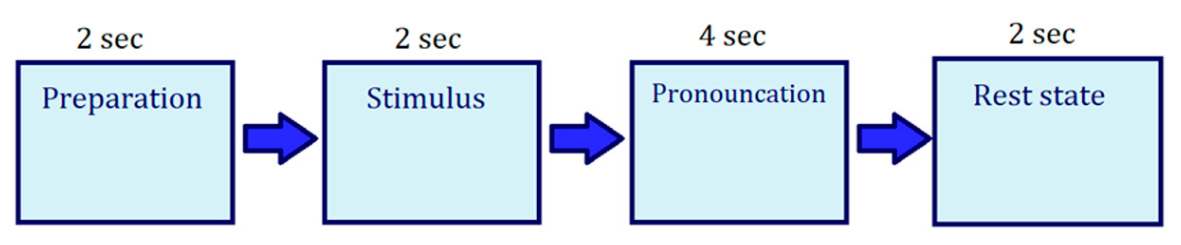
\includegraphics[width=0.7\linewidth]{images/recordingProtocol}
					\\ Fonte: \cite{tamm2020classification}
					\label{fig:recordingprotocol}
				\end{figure}
		\end{myenv}

	\chapter{Cronograma para conclusão do doutorado}
		\label{ch:cronograma}
		\begin{myenv}{1.5}
			\par Até a presente data foram realizados os levantamentos bibliográficos e o cumprimento dos créditos necessários em disciplinas para o Doutorado.
			\par Quanto aos trabalhos futuros os mesmo estão descritos na Tabela \ref{tb:cronograma}, porém primeiramente há que se separar o projeto em fases.
			
			\par A metodologia descrita é dividida em cinco etapas (E1 a E5) e tem como objetivo realizar um estudo sobre a aquisição e análise de \textit{imagined speech} por meio de eletroencefalografia (EEG) em locutores com dificuldades na fala.\newline
			
			\par \textbf{Na etapa E1}, foi realizado um levantamento bibliográfico sobre o estado-da-arte nas sub-áreas de aquisição e análise de \textit{imagined speech} por meio de EEG e de reconhecimento de voz em pacientes com disfonia. Foram estudados trabalhos publicados nas referências citadas na Seção \ref{sec:trabcorrelatos} e também cumpridos os créditos necessários das disciplinas do doutorado.\newline
			
			\par \textbf{Na etapa E2}, além de diálogos com profissionais das áreas de fonoaudiologia e neurologia. Também será estudada uma base de dados pública descrita em \cite{10.1117/12.2255697} para compreender os padrões comumente encontrados nos sinais de interesse. Por fim, será criada uma base de dados própria contendo sinais de voz verbalizados por locutores com dificuldades na fala, bem como sinais de EEG que possam conter representações das respectivas \textit{imagined speeches}. Será definido um conjunto de frases foneticamente ricas que serão lidas em voz alta pelos locutores voluntários. Os sinais acústicos serão capturados com um gravador eletrônico, enquanto os sinais de EEG serão capturados com eletrodos posicionados sobre o couro cabeludo dos voluntários.\newline
			
			\par \textbf{A etapa E3} envolverá o pré-processamento e a extração de características representativas para o objetivo proposto. Serão realizadas normalizações clássicas nos sinais, seguidas pela extração de características através de abordagens handcrafted e feature learning. A abordagem handcrafted envolverá a escolha de descritores guiados pela engenharia paraconsistente de características. Já a abordagem de feature learning investigará arquiteturas de redes neurais artificiais profundas projetadas para autocodificação. Serão extraídas características tanto dos sinais de voz quanto das \textit{imagined speeches}.\newline
			
			\par \textbf{A etapa E4} terá como foco a integração das etapas de extração de características (EC) e de autenticação. Serão empregadas estruturas de aprendizado profundo, como RNNs (Redes Neurais Recorrentes) e DSNNs (Deep Stacked Neural Networks), para o reconhecimento de padrões. Os resultados serão mensurados e comparados em termos de acurácia, levando em conta também o tempo de treinamento. Será realizada uma comparação entre as modalidades \textit{text-dependent} e \textit{text-independent}.\newline
			
			\par \textbf{A etapa E5} consistirá na apresentação dos experimentos em eventos científicos e na publicação dos resultados em periódicos de impacto. Também serão confeccionadas a monografia de qualificação e a tese de doutorado ao longo de todo o trabalho.
				
			\begin{table}[htbp]
				\label{tb:cronograma}
				\centering
				\definecolor{headerblue}{RGB}{0, 94, 184}
				\definecolor{lightgray}{RGB}{245, 245, 245}
				\renewcommand{\arraystretch}{1.5}
				
				\begin{minipage}{0.45\textwidth}
					\centering
					\rowcolors{2}{lightgray}{white}
					\begin{tabular}{|c|c|c|c|c|c|}
						\hline
						\rowcolor{headerblue}
						\textcolor{white}{Ms/Ano} & \textcolor{white}{E1} & \textcolor{white}{E2} & \textcolor{white}{E3} & \textcolor{white}{E4} & \textcolor{white}{E5} \\
						\hline
						09/22 & X & & & & \\
						10/22 & X & & & & \\
						11/22 & X & & & & \\
						12/22 & X & & & & \\
						01/23 & X & X & & & \\
						02/23 & X & X & & & \\
						03/23 & X & X & & & \\
						04/23 & X & X & & & \\
						05/23 & X & X & & & X \\
						06/23 & X & X & & & X \\
						07/23 & & X & X & & X \\
						08/23 & & X & X & & X \\
						09/23 & & X & X & & \\
						10/23 & & X & X & & \\
						11/23 & & X & X & & \\
						12/23 & & X & X & & \\
						01/24 & & X & X & X & X \\
						02/24 & & X & X & X & X \\
						03/24 & & & X & X & \\
						04/24 & & & X & X & \\
						05/24 & & & X & X & \\
						06/24 & & & X & X & \\
						07/24 & & & X & X & \\
						08/24 & & & X & X & \\
						\hline
					\end{tabular}
				\end{minipage}
				\hfill
				\begin{minipage}{0.45\textwidth}
					\centering
					\rowcolors{2}{lightgray}{white}
					\begin{tabular}{|c|c|c|c|c|c|}
						\hline
						\rowcolor{headerblue}
						\textcolor{white}{Mês/Ano} & \textcolor{white}{E1} & \textcolor{white}{E2} & \textcolor{white}{E3} & \textcolor{white}{E4} & \textcolor{white}{E5} \\
						\hline
						09/24 & & & X & X & \\
						10/24 & & & X & X & \\
						11/24 & & & X & X & \\
						12/24 & & & X & X & \\
						01/25 & & & X & X & \\
						02/25 & & & X & X & \\
						03/25 & & & X & X & \\
						04/25 & & & X & X & \\
						05/25 & & & X & X & \\
						06/25 & & & X & X & \\
						07/25 & & & X & X & \\
						08/25 & & & X & X & \\
						09/25 & & & X & X & \\
						10/25 & & & X & X & \\
						11/25 & & & X & X & \\
						12/25 & & & X & X & \\
						01/26 & & & X & X & \\
						02/26 & & & X & X & \\
						03/26 & & & X & X & \\
						04/26 & & & X & X & \\
						05/26 & & & & & X \\
						06/26 & & & & & X \\
						07/26 & & & & & X \\
						08/26 & & & & & X \\
						\hline
					\end{tabular}
				\end{minipage}
				\caption{Cronograma}
			\end{table}
	\end{myenv}

	\chapter{Apêndice}
	\label{ch:apendice}
	\begin{myenv}{1.5}
		\section{\textit{F1 score}}
		\label{sec:f1scoresec}
		\par O \textit{F1 score} é uma medida de desempenho utilizada em tarefas de classificação para avaliar o equilíbrio entre precisão e \textit{recall}. É uma métrica única que combina as duas medidas em um único valor, frequentemente usada quando lidamos com conjuntos de dados desbalanceados, nos quais a distribuição das classes é desigual.
		
		\par Para entender o \textit{F1 score}, vamos primeiro definir precisão e \textit{recall}:
		
		\begin{itemize}
			\item Precisão: Mede a proporção de instâncias positivas corretamente previstas (verdadeiros positivos) em relação a todas as instâncias previstas como positivas (verdadeiros positivos mais falsos positivos).
			
			\item \textit{Recall}: Mede a proporção de instâncias positivas corretamente previstas (verdadeiros positivos) em relação a todas as instâncias positivas reais (verdadeiros positivos mais falsos negativos). O \textit{recall} representa a capacidade do modelo de identificar todas as instâncias positivas.
		\end{itemize}
		
		\par Considerando isso o \textit{F1 score} é dados pela equação \ref{eq:f1score}:
		
		\begin{equation}
			\label{eq:f1score}
			\textit{F1 score} = 2 \times \frac{\textit{precisão} \times \textit{recall}}{\textit{precisão} + 	\textit{recall}}
		\end{equation}
		
		\par Essa métrica é considerada uma média harmônica, sendo assim, dá mais peso a valores mais baixos, fornecendo uma medida equilibrada que considera tanto a precisão quanto o \textit{recall}.
	\end{myenv}














	\bibliography{bibliography.bib}
	\bibliographystyle{alpha}

\end{document}

